
\chapter{第二章作业详细版}
\section{2 初边值的分离变量法}
\begin{homework}[1]
用分离变量法求下列定解问题的解：
\[
\begin{cases}
u_t=a^2u_{xx}, & t>0,\ 0<x<\pi,\\[4pt]
u(0,t)=0,\qquad u_x(\pi,t)=0, & t>0,\\[4pt]
u(x,0)=f(x), & 0<x<\pi.
\end{cases}
\]
\end{homework}
\begin{solution}
设 $u(x,t)=X(x)T(t)$，代入 $u_t=a^2u_{xx}$ 得
\[
\frac{T'}{a^2T}=\frac{X''}{X}=-\lambda.
\]
于是
\[
X''+\lambda X=0,\qquad T'+a^2\lambda T=0.
\]
边界条件给出
\[
X(0)=0,\qquad X'(\pi)=0.
\]
当 $\lambda=k^2>0$ 时，
\[
X(x)=A\sin kx+B\cos kx,\quad X(0)=0\Rightarrow B=0,
\]
\[
X'(x)=Ak\cos kx,\quad X'(\pi)=0\Rightarrow \cos(k\pi)=0
\Rightarrow k=\frac{2n-1}{2},\ n=1,2,\dots
\]
故本征函数
\[
X_n(x)=\sin\!\left(\frac{2n-1}{2}x\right),\qquad 
\lambda_n=\left(\frac{2n-1}{2}\right)^2.
\]
对应时间因子
\[
T_n(t)=e^{-a^2\lambda_n t}= \exp\!\left(-a^2\frac{(2n-1)^2}{4}\,t\right).
\]
因此解写为
\[
u(x,t)=\sum_{n=1}^{\infty}A_n
\sin\!\left(\frac{2n-1}{2}x\right)
\exp\!\left(-a^2\frac{(2n-1)^2}{4}\,t\right).
\]
由初值 $u(x,0)=f(x)$ 得 Fourier 系数
\[
f(x)=\sum_{n=1}^{\infty}A_n\sin\!\left(\frac{2n-1}{2}x\right),
\]
利用正交性
\[
\int_0^\pi \sin\!\left(\frac{2n-1}{2}x\right)\sin\!\left(\frac{2m-1}{2}x\right)\,dx
=\frac{\pi}{2}\delta_{mn},
\]
故
\[
A_n=\frac{2}{\pi}\int_0^\pi f(x)\sin\!\left(\frac{2n-1}{2}x\right)\,dx,
\qquad n=1,2,\dots
\]
\end{solution}
\begin{homework}[2]
用分离变量法求解热传导方程的初边值问题：
\[
\begin{cases}
\dfrac{\partial u}{\partial t}
= \dfrac{\partial^2 u}{\partial x^2}, & (t>0,\,0<x<1),\\[6pt]
u(x,0)=
\begin{cases}
x, & 0<x\le\dfrac{1}{2},\\[4pt]
1-x, & \dfrac{1}{2}<x<1,
\end{cases}\\[10pt]
u(0,t)=u(1,t)=0, & (t>0).
\end{cases}
\]
\end{homework}
\begin{solution}
 % 题 2
\[
u_t=u_{xx},\qquad u(0,t)=u(1,t)=0,\qquad 
u(x,0)=
\begin{cases}
x,&0<x\le \frac12,\\[2pt]
1-x,&\frac12<x<1
\end{cases}
\]

\[
u(x,t)=X(x)T(t)
\]

\[
\frac{T'}{T}=\frac{X''}{X}=-\lambda
\]

\[
T'+\lambda T=0,\qquad T(t)=C\,e^{-\lambda t}
\]

\[
X''+\lambda X=0,\qquad X(0)=X(1)=0
\]

\[
\lambda=(n\pi)^2,\qquad X_n(x)=\sin(n\pi x),\qquad n=1,2,\ldots
\]
\begin{dxtips}[正交系数]
    因为他已经写成了这样所以这个就是他的傅立叶展开式他的系数必须是傅立叶系数对吧
\end{dxtips}
\[
u(x,t)=\sum_{n=1}^{\infty}b_n\,e^{-(n\pi)^2 t}\,\sin(n\pi x)
\]

\[
b_n=2\int_{0}^{1}u(x,0)\sin(n\pi x)\,dx
=2\!\left(\int_{0}^{1/2}x\sin(n\pi x)\,dx+\int_{1/2}^{1}(1-x)\sin(n\pi x)\,dx\right)
\]

\[
\int x\sin(\alpha x)\,dx=-\frac{x\cos(\alpha x)}{\alpha}+\frac{\sin(\alpha x)}{\alpha^2}
\]

\[
b_n=\frac{2}{n\pi}\Bigl[-x\cos(n\pi x)\Bigr]_{0}^{1/2}
+\frac{2}{(n\pi)^2}\Bigl[\sin(n\pi x)\Bigr]_{0}^{1/2}
+\frac{2}{n\pi}\Bigl[-(1-x)\cos(n\pi x)\Bigr]_{1/2}^{1}
-\frac{2}{(n\pi)^2}\Bigl[\sin(n\pi x)\Bigr]_{1/2}^{1}
\]

\[
b_n=\frac{4}{(n\pi)^2}\,\sin\!\Bigl(\frac{n\pi}{2}\Bigr)
\]

\[
u(x,t)=\sum_{n=1}^{\infty}\frac{4}{\pi^2 n^2}\,\sin\!\Bigl(\frac{n\pi}{2}\Bigr)\,e^{-(n\pi)^2 t}\,\sin(n\pi x)
\]   
\end{solution}
\begin{definition}[傅立叶系数（常用三种情形）]
设 $f$ 为定义在区间上的可积函数，则其傅立叶系数定义如下：
\begin{itemize}
  \item \textbf{正弦级数（Dirichlet 边界）}  
  若
  \[
  f(x)=\sum_{n=1}^{\infty} b_n \sin\frac{n\pi x}{l},
  \qquad x\in(0,l),
  \]
  则其傅立叶正弦系数为
  \[
  b_n=\frac{2}{l}\int_0^l f(x)\sin\frac{n\pi x}{l}\,dx.
  \]

  \item \textbf{余弦级数（Neumann 边界）}  
  若
  \[
  f(x)=\frac{a_0}{2}+\sum_{n=1}^{\infty} a_n \cos\frac{n\pi x}{l},
  \qquad x\in(0,l),
  \]
  则其傅立叶余弦系数为
  \[
  a_0=\frac{2}{l}\int_0^l f(x)\,dx,
  \qquad
  a_n=\frac{2}{l}\int_0^l f(x)\cos\frac{n\pi x}{l}\,dx.
  \]

  \item \textbf{全傅立叶级数（周期情形）}  
  若
  \[
  f(x)=\frac{a_0}{2}+\sum_{n=1}^{\infty}
  \bigl(a_n\cos nx+b_n\sin nx\bigr),
  \qquad x\in(-\pi,\pi),
  \]
  则其傅立叶系数为
  \[
  a_n=\frac{1}{\pi}\int_{-\pi}^{\pi} f(x)\cos(nx)\,dx,
  \qquad
  b_n=\frac{1}{\pi}\int_{-\pi}^{\pi} f(x)\sin(nx)\,dx.
  \]
\end{itemize}
\end{definition}
\begin{note}
傅立叶正弦系数
\[
b_n=\frac{2}{l}\int_0^l f(x)\sin\frac{n\pi x}{l}\,dx
\]
可以理解为：

\begin{itemize}
  \item \textbf{方向匹配：}
  被积函数 $f(x)\sin\frac{n\pi x}{l}$ 表示
  $f$ 在第 $n$ 个正弦模态方向上的“相似程度”。

  \item \textbf{整体比较：}
  积分 $\displaystyle \int_0^l(\cdot)\,dx$ 表示在整个区间
  $(0,l)$ 上进行比较。

  \item \textbf{平均归一化：}
  系数前的 $\frac{2}{l}$ 来源于
  \[
  \int_0^l \sin^2\frac{n\pi x}{l}\,dx=\frac{l}{2},
  \]
  即除以正弦基函数自身的内积，使结果成为“平均值”。
\end{itemize}

因此，
\[
\boxed{\text{傅立叶正弦系数}
= \text{函数在对应正弦方向上的“平均投影强度”。}}
\]
\end{note}
\begin{dxtips}

 \begin{itemize}
  \item \textbf{分离变量原理}\\
  线性齐次偏微分方程在齐次边界条件下可以尝试形如
  $u(x,t)=X(x)T(t)$ 的乘积解，从而将 PDE 化为两个常微分方程。

  \item \textbf{自伴随算子的特征值问题}\\
  空间算子 $L[X]=X''$ 加齐次狄利克雷边界条件 $X(0)=X(1)=0$ 构成
  Sturm–Liouville 系统，其特征值与特征函数为
  \[
    \lambda_n=(n\pi)^2,\qquad X_n(x)=\sin(n\pi x).
  \]

  \item \textbf{正交基展开原理}\\
  $\{\sin(n\pi x)\}_{n\ge1}$ 作为 Sturm–Liouville 系统的特征函数，
  在 $L^2(0,1)$ 中构成一组完备正交基，可用于展开任意初始函数
  $f\in L^2(0,1)$。

  \item \textbf{傅里叶正弦级数的系数公式}\\
  基于正交性
  \[
    \int_0^1 \sin(n\pi x)\sin(m\pi x)\,dx = \frac12\delta_{mn},
  \]
  得到初始条件展开系数
  \[
    b_n = 2\int_0^1 f(x)\sin(n\pi x)\,dx.
  \]

  \item \textbf{线性叠加与唯一性原理}\\
  对线性齐次 PDE，所有特征解的级数叠加仍是解；
  热方程满足适定性与唯一性，故由级数展开得到的解即为唯一解。

\end{itemize}
\end{dxtips}
\section{3柯西问题}
% 约定：对 $f\in L^1(\mathbb R)$ 定义一维傅里叶变换
% \[
%   \mathcal F[f](\omega)=\hat f(\omega)
%   =\int_{-\infty}^{\infty}f(x)e^{-i\omega x}\,dx .
% \]

%------------------ 题 1 ------------------%
\begin{homework}[1]
求下列函数的傅里叶变换：
\begin{enumerate}[(1)]
  \item $e^{-\eta x^2}\quad(\eta>0)$；
  \item $e^{-a|x|}\quad(a>0)$；
  \item $\displaystyle\frac{x}{(a^2+x^2)^k},\qquad
        \frac1{(a^2+x^2)^k}\quad(a>0,\;k\in\mathbb N)$。
\end{enumerate}
\end{homework}
\begin{dxtips}
    \begin{itemize}
  \item 基本高斯积分（母本）：
  \[
    \int_{-\infty}^{\infty} e^{-x^2}\,dx = \sqrt{\pi}.
  \]
  \item 缩放规则：令 $y=\sqrt{\eta}\,x$，则
  \[
    \int_{-\infty}^{\infty} e^{-\eta x^2}\,dx
      = \frac{1}{\sqrt{\eta}}
        \int_{-\infty}^{\infty} e^{-y^2}\,dy
      = \sqrt{\frac{\pi}{\eta}},\quad \eta>0.
  \]
  \item 平移不改变值：
  \[
    \int_{-\infty}^{\infty} e^{-\eta (x-\mu)^2}\,dx
    = \sqrt{\frac{\pi}{\eta}}.
  \]
  \item 一般二次型（完全平方后套用）：
  \[
    \int_{-\infty}^{\infty} e^{-(ax^2+bx+c)}\,dx
    = e^{\frac{b^2}{4a}-c}\sqrt{\frac{\pi}{a}},\quad a>0.
  \]
\end{itemize}
\end{dxtips}
\begin{note}
    配平方的目的就是把含有x的项都去掉，用高斯积分套公式，剩下的常数提取到积分外面就行不碍事
\end{note}
\begin{solution}
(1) 经典高斯积分给出
\[
\int_{-\infty}^{\infty}e^{-\eta x^2}\,dx=\sqrt{\frac{\pi}{\eta}},
\]
于是
\[
\hat f(\omega)
=\int_{-\infty}^{\infty}e^{-\eta x^2}e^{-i\omega x}\,dx
=\sqrt{\frac{\pi}{\eta}}\,
   e^{-\frac{\omega^2}{4\eta}},\qquad \eta>0 .
\]

(2) 先在 $x>0$ 与 $x<0$ 分别积分：
\[
\hat f(\omega)
=\int_{-\infty}^{\infty}e^{-a|x|}e^{-i\omega x}\,dx
=\int_{0}^{\infty}e^{-(a+i\omega)x}\,dx
   +\int_{0}^{\infty}e^{-(a-i\omega)x}\,dx
=\frac1{a+i\omega}+\frac1{a-i\omega}
=\frac{2a}{a^2+\omega^2}.
\]

(3) 先回忆 $k=1$ 的情形：
\[
\frac1{a^2+x^2}
\quad\Longleftrightarrow\quad
\frac{\pi}{a}e^{-a|\omega|}.
\]
对参数 $a$ 作导数可得到高次幂：
\[
\frac1{(a^2+x^2)^k}
=\frac{(-1)^{k-1}}{(k-1)!}\,
  \frac{\partial^{k-1}}{\partial a^{\,k-1}}
  \frac1{a^2+x^2},
\]
因此
\[
\mathcal F\!\left[\frac1{(a^2+x^2)^k}\right](\omega)
=\frac{(-1)^{k-1}}{(k-1)!}\,
  \frac{\partial^{k-1}}{\partial a^{\,k-1}}
  \left(\frac{\pi}{a}e^{-a|\omega|}\right),
  \qquad k\in\mathbb N.
\]

再利用性质
\[
\mathcal F[xg(x)](\omega)
=i\,\frac{d}{d\omega}\hat g(\omega),
\]
令 $g(x)=(a^2+x^2)^{-k}$，即可得到
\[
\mathcal F\!\left[\frac{x}{(a^2+x^2)^k}\right](\omega)
=i\,\frac{d}{d\omega}
\left\{
\frac{(-1)^{k-1}}{(k-1)!}\,
  \frac{\partial^{k-1}}{\partial a^{\,k-1}}
  \left(\frac{\pi}{a}e^{-a|\omega|}\right)
\right\}.
\]
上述给出了一般 $k$ 的显式表达（是 $|\omega|$ 的多项式乘
$e^{-a|\omega|}$）。
\end{solution}
\begin{dxtips}
    因为要保证z=z0的时候 左边就只剩下留数不是0所以两边先乘 z的m阶导 此时留数的后面跟着z-z0的m减1要去掉z-z0来保证留数能留下所以要导m-1次
\end{dxtips}
\begin{dxtips}
\begin{enumerate}
  \item 要背基础式子：
  $$
  \mathcal F\left[\frac{1}{a^{2}+x^{2}}\right](\omega)
    = \frac{\pi}{a}\,e^{-a|\omega|}.
  $$

  \item $k$ 次方和一次方之间的关系：
  $$
  \frac{1}{(a^{2}+x^{2})^{k}}
    = \frac{(-1)^{k-1}}{(k-1)!\,2^{\,k-1}a^{\,k-1}}
      \frac{\partial^{\,k-1}}{\partial a^{\,k-1}}
      \left(\frac{1}{a^{2}+x^{2}}\right),
    \qquad k\in\mathbb N.
  $$

  \item 利用“对参数 $a$ 的求导可以与傅里叶积分号交换”，
  在计算
  $
  \mathcal F\left[\frac{1}{(a^{2}+x^{2})^{k}}\right]
  $
  时，可以把对 $a$ 的高阶导数先提到积分号外面，
  这样积分内部始终只含有母式
  $
  \frac{1}{a^{2}+x^{2}}.
  $

  \item 乘以 $x$ 的傅里叶变换公式：
  $$
  \mathcal F\big[x\,g(x)\big](\omega)
    = i\,\frac{d}{d\omega}\,\hat g(\omega).
  $$
\end{enumerate}
    
\end{dxtips}

%------------------ 题 2 ------------------%
\begin{homework}[2]
设 $f(x)$ 在 $(-\infty,\infty)$ 绝对可积，证明其傅里叶变换
\[
\hat f(\omega)=\int_{-\infty}^{\infty}f(x)e^{-i\omega x}\,dx
\]
是连续函数。
\end{homework}
\begin{dxtips}
    \begin{itemize}
  \item \textbf{(1) $L^1(\mathbb R)$ 的定义与性质}\\
  绝对可积函数形成的空间；可积函数与平移、控制函数相关的一切都建立在 $L^1$ 的基本性质上。

  \item \textbf{(2) 指数函数 $e^{-i\omega x}$ 对 $\omega$ 的连续性}\\
  对每个固定 $x$，有 $e^{-i\omega x}\to e^{-i\omega_0 x}$，且模长恒为 1。

  \item \textbf{(3) 受控收敛定理（Dominated Convergence Theorem）}\\
  用统一可积的 majorant（这里是 $|f(x)|$）控制被积函数族，从而允许把极限移入积分号。
\end{itemize}
\end{dxtips}
\begin{solution}
任取 $\omega_0\in\mathbb R$，令 $\omega\to\omega_0$。有
\[
\hat f(\omega)-\hat f(\omega_0)
=\int_{-\infty}^{\infty}
  f(x)\bigl(e^{-i\omega x}-e^{-i\omega_0 x}\bigr)\,dx .
\]
于是
\[
\bigl|\hat f(\omega)-\hat f(\omega_0)\bigr|
\le\int_{\mathbb R}|f(x)|\,
   \bigl|e^{-i\omega x}-e^{-i\omega_0 x}\bigr|\,dx
\le 2\int_{\mathbb R}|f(x)|\,dx<\infty.
\]

对每个固定的 $x$，当 $\omega\to\omega_0$ 时，
$e^{-i\omega x}\to e^{-i\omega_0 x}$，因此
\[
f(x)\bigl(e^{-i\omega x}-e^{-i\omega_0 x}\bigr)
\to 0 .
\]
又因为
\[
\bigl|f(x)(e^{-i\omega x}-e^{-i\omega_0 x})\bigr|
\le 2|f(x)|,\qquad 2|f(x)|\in L^1(\mathbb R),
\]
由支配收敛定理可得
\[
\lim_{\omega\to\omega_0}
\bigl(\hat f(\omega)-\hat f(\omega_0)\bigr)
=\int_{\mathbb R}
  \lim_{\omega\to\omega_0}
  f(x)\bigl(e^{-i\omega x}-e^{-i\omega_0 x}\bigr)\,dx
=0.
\]
故 $\hat f(\omega)$ 在任意点 $\omega_0$ 处连续，即 $\hat f$ 为连续函数。
\end{solution}

\begin{dxtips}
    要证明连续先要选w0属于R，w趋紧于w0时f(w)趋紧于f（w0），我们都目的是为了把极限符号从积分外面弄到积分里面让他可以作用到$\bigl(e^{-i\omega x}-e^{-i\omega_0 x}\bigr)\,dx
=0.$,为了这个目的我们要做两件事第一点态收敛因为对于确定的x，f(x)$\bigl(e^{-i\omega x}-e^{-i\omega_0 x}\bigr)\,dx
=0.$,当w0趋紧w时天然成立。然后就是要证明
$
\bigl|f(x)(e^{-i\omega x}-e^{-i\omega_0 x})\bigr|
\le 2|f(x)|,\qquad 2|f(x)|\in L^1(\mathbb R),
$有上界因为只含e的项相当于默认模长就是1，因为e的哪一项只是旋转角度。所以找出连上界他们就可以交换lim然后就完成证明了
\end{dxtips}
%------------------ 题 3 ------------------%
\begin{homework}[3]
用傅里叶变换求解三维热传导方程的柯西问题
\[
\begin{cases}
\dfrac{\partial u}{\partial t}
=a^2\left(
\dfrac{\partial^2 u}{\partial x^2}
+\dfrac{\partial^2 u}{\partial y^2}
+\dfrac{\partial^2 u}{\partial z^2}
\right),
& t>0,\ (x,y,z)\in\mathbb R^3,\\[6pt]
u(x,y,z,0)=\varphi(x,y,z),
& (x,y,z)\in\mathbb R^3.
\end{cases}
\]
\end{homework}

\begin{solution}
对空间变量 $(x,y,z)$ 作三维傅里叶变换。记
\[
\hat u(\boldsymbol\xi,t)
=\mathcal F_{x,y,z}[u](\boldsymbol\xi,t),
\qquad\boldsymbol\xi=(\xi_1,\xi_2,\xi_3),
\]
则
\[
\mathcal F\!\left[\frac{\partial u}{\partial t}\right]
=\frac{\partial\hat u}{\partial t},\qquad
\mathcal F[u_{xx}+u_{yy}+u_{zz}]
=-(\xi_1^2+\xi_2^2+\xi_3^2)\hat u .
\]
于是原方程化为常微分方程
\[
\frac{\partial\hat u}{\partial t}
=-a^2|\boldsymbol\xi|^2\hat u,
\qquad
\hat u(\boldsymbol\xi,0)=\hat\varphi(\boldsymbol\xi),
\]
解得
\[
\hat u(\boldsymbol\xi,t)
=\hat\varphi(\boldsymbol\xi)\,
  e^{-a^2|\boldsymbol\xi|^2 t}.
\]

再取三维反傅里叶变换，
\[
u(x,y,z,t)
=\mathcal F^{-1}\!\Bigl[
   \hat\varphi(\boldsymbol\xi)\,
   e^{-a^2|\boldsymbol\xi|^2 t}
 \Bigr]
=\bigl(G(\cdot,t)*\varphi\bigr)(x,y,z),
\]
其中 $*$ 为 $\mathbb R^3$ 上的卷积，$G$ 为三维热核
\[
G(x,y,z,t)
=\frac1{(4\pi a^2 t)^{3/2}}
  \exp\!\left(
   -\frac{x^2+y^2+z^2}{4a^2 t}
  \right),\qquad t>0.
\]

因此所求解为
\[
u(x,y,z,t)
=\frac1{(4\pi a^2 t)^{3/2}}
  \int_{\mathbb R^3}
  \exp\!\left(
   -\frac{(x-\xi)^2+(y-\eta)^2+(z-\zeta)^2}{4a^2 t}
  \right)
  \varphi(\xi,\eta,\zeta)\,d\xi\,d\eta\,d\zeta .
\]
\end{solution}
\begin{dxtips}
    \begin{enumerate}
  \item \textbf{母式 A：傅里叶对导数的公式}
  \[
    \mathcal{F}[\Delta u](\xi) = -|\xi|^{2}\,\hat{u}(\xi),
  \]
  也就是说，“拉普拉斯算子在频域里就变成乘上 $-|\xi|^{2}$”。

  \item \textbf{母式 B：高斯的傅里叶变换（热核母式）}
  \[
    \mathcal{F}^{-1}_{\xi\to x}\!\left(e^{-a^{2}|\xi|^{2}t}\right)
    = \frac{1}{(4\pi a^{2}t)^{3/2}}
      \exp\!\left(-\frac{|x|^{2}}{4a^{2}t}\right).
  \]
\end{enumerate}
% 一维情形下，傅里叶变换与导数的关系：
\end{dxtips}
\begin{dxtips}

母式B和最开头的高斯积分有关

\[
\mathcal{F}[u_x](\xi) = i\xi\,\hat u(\xi), \qquad
\mathcal{F}[u_{xx}](\xi) = (i\xi)^2 \hat u(\xi) = -\xi^2 \hat u(\xi).
\]

也就是说，在“傅里叶的世界”里，对 $x$ 求一次导数
\[
u_x \quad \xrightarrow{\ \mathcal{F}\ }\quad i\xi\,\hat u(\xi),
\]
再求一次导数
\[
u_{xx} \quad \xrightarrow{\ \mathcal{F}\ }\quad (i\xi)^2\hat u(\xi)=-\xi^2\hat u(\xi),
\]
即\textbf{“在傅里叶的世界里，对 $x$ 的求导就是乘上 $i\xi$（两次导就是乘 $(i\xi)^2$）”}。

\end{dxtips}
\begin{dxtips}
    x是空间位置，\xi是频率变量 sinnx，cosnx，n类似\xi, \xi就是连续的n（角速度？），\xi 就是一个变量一个符号不需要知道是多少，先固定\xi把\xi 当常数，解完了对所有的都有效。
\end{dxtips}
\section{4极值原理，定解问题解的唯一性和稳定性}
p93
\begin{homework}[2]
利用证明热传导方程极值原理的方法，证明：满足方程
\[
\frac{\partial^2 u}{\partial x^2}+\frac{\partial^2 u}{\partial y^2}=0
\]
的函数在有界闭区域上的最大值不超过它在边界上的最大值。
\end{homework}
\begin{definition}[调和函数]
设 $\Omega\subset\mathbb R^n$ 是开集。函数 $u:\Omega\to\mathbb R$
若在 $\Omega$ 上二阶连续可微，且满足
\[
\Delta u(x)
:= \sum_{j=1}^n \frac{\partial^2 u}{\partial x_j^2}(x) = 0,
\qquad x\in\Omega,
\]
则称 $u$ 为 $\Omega$ 上的\textbf{调和函数}。
\end{definition}
\begin{itemize}
  \item \textbf{几何意义：}\\
  在二维，
  \[
    \Delta u = u_{xx} + u_{yy},
  \]
  在三维，
  \[
    \Delta u = u_{xx} + u_{yy} + u_{zz}.
  \]
  可以把拉普拉斯算子看成“各个坐标方向上弯曲程度（二阶导数）的总和”：整体上
  \(\Delta u>0\) 像“盆地”，\(\Delta u<0\) 像“山包”。

  \item \textbf{与周围平均值的关系：}\\
  在某一点 \(x_0\) 处，
  \(\Delta u(x_0)\) 与“周围小球上的平均值减去中心值”成正比：大致有
  \[
    \Delta u(x_0) \propto
    \frac{\text{小球边界上的平均值} - u(x_0)}{\text{半径}^2}.
  \]
  因此
  \(\Delta u>0\) 表示周围平均值比中心大（中心偏低），
  \(\Delta u<0\) 表示周围平均值比中心小（中心偏高）。

  \item \textbf{在热传导 / 扩散中的物理意义：}\\
  对热方程
  \[
    u_t = a^2 \Delta u,
  \]
  这里 \(u(x,t)\) 是温度，\(u_t\) 是温度随时间的变化率，
  \(\Delta u\) 则刻画该点温度相对于周围的“失衡程度”：
  \begin{itemize}
    \item \(\Delta u>0\)：该点比周围冷，热量从周围向这里流入，温度上升；
    \item \(\Delta u<0\)：该点比周围热，热量从这里向外流出，温度下降；
    \item \(\Delta u=0\)：该点温度等于周围平均值，本地没有净流入/流出，处于局部平衡。
  \end{itemize}

  \item \textbf{与调和函数的关系：}\\
  调和函数满足
  \[
    \Delta u = 0.
  \]
  物理上可以理解为：在这样的场里，任何一点都没有“净源”或“净汇”，
  即没有净产生或净消失。比如：
  \begin{itemize}
    \item 静电学中：无电荷区域的电势满足 \(\Delta u=0\)；
    \item 稳态热传导中：没有热源和散热片的区域，温度场满足 \(\Delta u=0\)。
  \end{itemize}
  这也解释了调和函数的平均值性质和最大值原理：
  点值等于周围平均值，内部不能出现孤立尖峰的真正极大值。
\end{itemize}
\begin{dxtips}
    证明思路，只分两种情况一边界值上本了就是最大值，这个就符合题目要求了，第二也就是中心某一点取到最大值，最大值是极致点对x，y对一节倒数等于0，二阶导数小于等于0，但是这里说了二阶导数之和恒等于0，唯一满足的就是二阶导数也都是0。然后根据两个偏导都是零，调和函数性质他的领域内都是M，他的临域都是M那么这些点的临域还是M\\
    下面那句“在 $(x_0,y_0)$ 的某邻域内有……由上述推出 $u(x,y)\equiv M$ 于该邻域”，
实际上是用到了调和函数的\textbf{强最大值原理}（或平均值性质）。可以这样理解：

\begin{itemize}
  \item 因为 $u_{xx}+u_{yy}=0$ 且 $(x_0,y_0)$ 是内点最大值点，
  在某个小邻域 $U$ 里始终有
  \[
    u(x,y)\le u(x_0,y_0)=M,\qquad u_{xx}+u_{yy}=0.
  \]

  \item 对调和函数 $u$，我们有\textbf{平均值性质}：
  某一点的值等于该点周围小圆上的平均值。
  如果这点的取值是最大值 $M$，而周围所有点的值都 $\le M$，
  那么这个“平均值”只有在圆上所有点都等于 $M$ 时才能仍然是 $M$；
  否则平均值会小于 $M$，与中心点取到最大值矛盾。

  \item 所以结论是：在这个小邻域 $U$ 内，必须有
  \[
    u(x,y)\equiv M.
  \]
\end{itemize}

也就是说：一旦调和函数在内部某点取得最大值，它在该点附近就只能是常数。
这就是\textbf{强最大值原理}的局部版本。
\end{dxtips}
\begin{dxtips}
    \begin{itemize}
  \item \textbf{调和函数的定义}\\
  $u\in C^2(\Omega)$ 且满足
  \[
    u_{xx}+u_{yy}=0 \quad\text{（Laplace 方程）},
  \]
  则称 $u$ 为调和函数。

  \item \textbf{内部极值的二阶必要条件}\\
  若 $u$ 在内部点取得极大值，则
  \[
    u_x=u_y=0,\qquad 
    u_{xx}\le 0,\; u_{yy}\le 0.
  \]

  \item \textbf{对调和函数的二阶约束}\\
  调和条件给出
  \[
    u_{xx}+u_{yy}=0,
  \]
  与上条结合推出
  \[
    u_{xx}=u_{yy}=0.
  \]

  \item \textbf{最大值原理的关键推论}\\
  若调和函数在内部某点 $(x_0,y_0)$ 取得真最大值，则在该点附近满足
  \[
    u(x,y)\le u(x_0,y_0),\qquad
    u_{xx}+u_{yy}=0,
  \]
  从而可推出
  \[
    u\equiv \text{常数}.
  \]

  \item \textbf{得出最大值原理}\\
  非常数调和函数不可能在内部取得最大值，因此
  \[
    \max_{\overline\Omega} u = \max_{\partial\Omega} u.
  \]
\end{itemize}
\end{dxtips}
\begin{solution}
设 $\overline\Omega$ 为有界闭区域，$u\in C^2(\Omega)\cap C(\overline\Omega)$，满足
\[
u_{xx}+u_{yy}=0\quad\text{于 }\Omega.
\]

记
\[
M=\max_{\overline\Omega}u.
\]

若 $M$ 在 $\partial\Omega$ 取得，则
\[
\max_{\overline\Omega}u=\max_{\partial\Omega}u.
\]

若 $M$ 在内部点 $(x_0,y_0)\in\Omega$ 处取得，则
\[
u_x(x_0,y_0)=u_y(x_0,y_0)=0,
\]
\[
u_{xx}(x_0,y_0)\le0,\qquad u_{yy}(x_0,y_0)\le0,
\]
从而
\[
u_{xx}(x_0,y_0)+u_{yy}(x_0,y_0)\le0.
\]
而
\[
u_{xx}(x_0,y_0)+u_{yy}(x_0,y_0)=0,
\]
故
\[
u_{xx}(x_0,y_0)=u_{yy}(x_0,y_0)=0.
\]

在 $(x_0,y_0)$ 的某邻域内有
\[
u(x,y)\le u(x_0,y_0)=M,\qquad
u_{xx}(x,y)+u_{yy}(x,y)=0,
\]
由上式推出
\[
u(x,y)\equiv M\quad\text{于该邻域},
\]
从而
\[
u(x,y)\equiv M\quad\text{于 }\Omega,
\]
故
\[
\max_{\overline\Omega}u=\max_{\partial\Omega}u.
\]
\end{solution}
\begin{homework}[3]
设 $u(x,t)$ 为热传导方程
\[
u_t - a^2 u_{xx} - c u = 0,\qquad c>0,
\]
在矩形区域
\[
R=\{(x,t)\mid 0 < x < l,\ 0<t<T\}
\]
中的解。

已知：
\[
|u(0,t)|,\ |u(l,t)| \le M,\qquad t\in[0,T],
\]
\[
|u(x,0)|\le M,\qquad x\in[0,l].
\]

试证：
\[
|u(x,t)|\le M e^{ct},\qquad (x,t)\in R.
\]
\end{homework}
\begin{dxtips}
    \textbf{(1) 目标}：原方程
\[
u_t-a^2u_{xx}-cu=0
\]
多了一个 $-cu$ 项，想通过变换把它化为标准热方程
\[
v_t-a^2v_{xx}=0,
\]
以便套用最大值原理估计解。

\medskip
\textbf{(2) 指数变换去掉 $-cu$ 项}：令
\[
v(x,t)=u(x,t)e^{-ct},
\]
则
\[
v_t=u_t e^{-ct}-cu e^{-ct},\qquad v_{xx}=u_{xx}e^{-ct}.
\]
由原方程得
\[
u_t-cu=a^2u_{xx},
\]
代入上式：
\[
v_t=(u_t-cu)e^{-ct}=a^2u_{xx}e^{-ct}=a^2v_{xx},
\]
即
\[
v_t-a^2v_{xx}=0.
\]
因此，通过乘以 $e^{-ct}$，我们把带有 $-cu$ 的方程成功化为标准热方程。```
\end{dxtips}
\begin{solution}
令
\[
v(x,t)=u(x,t)e^{-ct}.
\]
则
\[
v_t = u_t e^{-ct} - c u e^{-ct},\qquad
v_{xx} = u_{xx} e^{-ct}.
\]
由原方程
\[
u_t-a^2u_{xx}-cu=0
\]
可得
\[
u_t - cu = a^2 u_{xx}.
\]
代入上式，有
\[
v_t = (u_t - cu)e^{-ct} = a^2 u_{xx}e^{-ct} = a^2 v_{xx},
\]
即
\[
v_t - a^2 v_{xx} = 0.
\]
因此 $v$ 在矩形区域
\[
R=\{(x,t)\mid 0<x<l,\ 0<t<T\}
\]
内满足标准热传导方程。

再看边界条件：

- 当 $x=0,l$ 时，
  \[
  |v(0,t)| = |u(0,t)|e^{-ct}\le M e^{-ct}\le M,\qquad
  |v(l,t)| = |u(l,t)|e^{-ct}\le M e^{-ct}\le M,\quad t\in[0,T].
  \]
- 当 $t=0$ 时，
  \[
  v(x,0)=u(x,0),\qquad |v(x,0)|=|u(x,0)|\le M,\quad x\in[0,l].
  \]

因此，在区域 $R$ 的抛物型边界上，
\[
|v(x,t)|\le M.
\]

由热方程的最大值原理（对 $v$ 和 $-v$ 都适用），可知在整个区域 $R$ 内
\[
|v(x,t)|\le M,\qquad (x,t)\in R.
\]
于是
\[
|u(x,t)| = |v(x,t)|e^{ct} \le M e^{ct},\qquad (x,t)\in R,
\]
即所要证明的结论。
\end{solution}
\begin{dxtips}
    我明白了所以这个题因为给的是边界条件所以要让式子变成基础的才能用最大值原理，所以要把u换成v一个是为了消除c另一个就是为了可以用最大原理.这个给了边界条件要求证明没一点每一个时刻都符合
    最大值原理（口语版）
如果 w 在矩形区域 R 里满足基础热方程，并且在抛物边界上连续，
那么 w 在闭区域 \overline R 的最大值一定出现在边界上，
不会在内部诡异地突然长出一个更大的峰值。

\end{dxtips}

\begin{homework}[5]
设 $u(x,t)$ 是区域 $\{0\le x\le \pi,\ 0\le t<\infty\}$ 中问题的经典解：
\[
\begin{cases}
u_t=u_{xx},\\[4pt]
u_x|_{x=0}=u_x|_{x=\pi}=0,\\[4pt]
u|_{t=0}=\varphi(x),
\end{cases}
\]
其中 $\varphi(0)=\varphi'(\pi)=0$。

证明：
\[
\sup_{0<x<\pi}|u(x,1)|\ \le\ \sup_{0<x<\pi}|\varphi(x)|.
\]

\textit{提示：将函数 $u(x,t)$ 关于直线 $x=\pi$ 作偶延拓到 $x\in(\pi,2\pi)$ 中。}
\end{homework}
\begin{dxtips}[证明目的]
    带 Neumann 边界条件 $u_x(0,t)=u_x(\pi,t)=0$ 和初始条件 $u(x,0)=\varphi(x)$（且 $\varphi(0)=\varphi'(\pi)=0$）的经典解 $u(x,t)$ 中，在时刻 $t=1$ 的解的最大绝对值，不会超过初始函数 $\varphi$ 的最大绝对值，即
\[
\sup_{0<x<\pi} |u(x,1)| \le \sup_{0<x<\pi} |\varphi(x)|.
\]
\end{dxtips}

\begin{dxtips}
    一看见比大小的就要想到极大值原理
\end{dxtips}
\begin{dxtips}
    关于 $C$ 其实就是因为要用绝对值，所以它上下界都得确定，然后把 $C$ 作为一个固定常数，要把 $C$ 从限制 $t=0$ 时刻推广到限制每一个时刻，具体做法就是：先选一个常数 $C\ge \sup|\psi|$，这样只保证在初始时刻 $t=0$ 有 $|v(x,0)|\le C$；然后构造两个新函数 $v_C^{+}=v-C$ 和 $v_C^{-}=-v-C$，让它们在 $t=0$ 时都满足 $v_C^{\pm}(x,0)\le 0$，并且同样满足热方程和相应的边界条件，这样就可以对 $v_C^{\pm}$ 使用最大值原理：既然它们在底边（加上通过偶延拓处理后的侧边）都不大于 $0$，那么在所有 $0<t\le1$ 的时刻也都不可能大于 $0$。把这个结论翻译回去，就是对每一个时刻都有 $-C\le v(x,t)\le C$，也就是 $|v(x,t)|\le C$，从而把原本只在 $t=0$ 成立的“$|v|\le C$”推广到了整个时间区间。
\end{dxtips}
\begin{dxtips}
    v是延拓完了的u在t=0时=\psi(x)
    对，可以这么总结成一段话：

这题的关键是想用极值原理说明：在我们关心的矩形里，解的最大值只能来自底边 t=0 上的初始函数，而不会在后面的时间或侧边上产生新的更大值。为此先把原来的解 u 在 0≤x≤π 上按 x=π 做偶延拓，得到在 0≤x≤2π 上的 v。这样原来可能在 x=0、x=π 这两条 Neumann 边界上出现的极大值，被“拉进”了更大的区间内部点，但 v 依然满足热方程和相应的光滑性条件，所以仍然可以应用热方程的极大值原理：内部不能产生新的正极大值。于是极大值只能来自底边 t=0。接下来再讨论 t=0 时的情况：选一个常数 C 大于等于初始函数绝对值的上确界，构造 v−C 和 −v−C，这两个函数在 t=0 底边上都不大于 0，由极大值原理可知在整个区域内也都不大于 0，从而得到 |v(x,t)|≤C，特别在 t=1 时 |v(x,1)|≤C，再用 C≥sup|φ| 就得到题目要求的不等式。
\end{dxtips}
\begin{solution}
\text{在 }0\le x\le\pi\text{ 上：}\quad
\begin{cases}
u_t=u_{xx},\\
u_x(0,t)=u_x(\pi,t)=0,\\
u(x,0)=\varphi(x).
\end{cases}

\text{偶延拓到 }(0,2\pi):\quad
v(x,t)=
\begin{cases}
u(x,t), & 0\le x\le\pi,\\[2mm]
u(2\pi-x,t), & \pi\le x\le2\pi.
\end{cases}
\]

则
\[
v_t=v_{xx},\qquad v_x(0,t)=v_x(2\pi,t)=0,
\]
\[
v(x,0)=\psi(x):=
\begin{cases}
\varphi(x), & 0\le x\le\pi,\\[1mm]
\varphi(2\pi-x), & \pi\le x\le2\pi,
\end{cases}
\]
\[
\sup_{0<x<2\pi}|\psi(x)|=\sup_{0<x<\pi}|\varphi(x)|.
\]

\[
v_C^{+}(x,t)=v(x,t)-C,\qquad 
v_C^{-}(x,t)=-v(x,t)-C.
\]

\[
(v_C^{+})_t=(v_C^{+})_{xx},\qquad
(v_C^{-})_t=(v_C^{-})_{xx}.
\]

\[
v_C^{+}(x,0)=\psi(x)-C\le 0,\qquad
v_C^{-}(x,0)=-\psi(x)-C\le 0,
\]
\[
\text{当 } C\ge \sup_{0<x<2\pi}|\psi(x)|\text{ 时成立}.
\]

由热方程最大值原理得
\[
v_C^{\pm}(x,t)\le0\quad(0<x<2\pi,\ 0<t\le1),
\]
即
\[
|v(x,1)|\le C\quad(0<x<2\pi).
\]

令
\[
C=\sup_{0<x<2\pi}|\psi(x)|=\sup_{0<x<\pi}|\varphi(x)|,
\]
得
\[
|v(x,1)|\le\sup_{0<x<\pi}|\varphi(x)|,\qquad 0<x<2\pi.
\]

对 $0<x<\pi$，有 $v(x,1)=u(x,1)$，故
\[
\sup_{0<x<\pi}|u(x,1)|
\le\sup_{0<x<\pi}|\varphi(x)|.
\]
\end{solution}
\begin{dxtips}
    偶延拓就是把函数按照x=π对称过去
    本质是要排除极值在侧边的可能性。就是延拓了以后右侧边和对称的左侧遍都算内部了，然后他依然保持着能用最大值原理的条件然后就证明了最大值只能再底边
    \begin{itemize}
  \item 底边：$t=0,\ \alpha\le x\le\beta$，这条边上给的就是
  \[
    u(x,0)=\varphi(x),
  \]
  所以 $\varphi(x)$ 就对应这条底边（也叫“初始边”、“初始线”）。

  \item 左侧边：$x=\alpha,\ 0\le t\le T$。

  \item 右侧边：$x=\beta,\ 0\le t\le T$。
\end{itemize}
\end{dxtips}    
\begin{note}
    取常数 $C$，使得
\[
C \;\ge\; \sup_{0<x<2\pi} |\psi(x)|
  \;=\; \sup_{0<x<\pi} |\varphi(x)|,
\]
即 $C$ 是一个不小于初始函数绝对值上确界的常数。
\end{note}
\section{12.1 5解的渐进太}
95
\begin{dxtips}[必背公式-热核公式]
更一般的 $n$ 维热核是：
\[
G_n(x,t)
=\frac{1}{(4\pi a^{2}t)^{n/2}}
   \exp\!\left(-\frac{|x|^{2}}{4a^{2}t}\right),\qquad x\in\mathbb{R}^n.
\]

二维只是把 $n=2$ 代进去。    
\end{dxtips}
\begin{homework}[2]
证明：当 $\varphi(x,y)$ 为 $\mathbb R^2$ 上的有界连续函数，且 $\varphi\in L^1(\mathbb R^2)$ 时，二维热传导方程柯西问题的解，当 $t\to\infty$ 时，以 $t^{-1}$ 衰减率趋于零。
\end{homework}
\begin{theorem}[热方程柯西问题的基本解表示]
设 $\varphi\in L^{1}(\mathbb{R}^{n})$ 有界且连续，考虑 $n$ 维热传导方程的柯西问题
\[
\begin{cases}
u_t-a^{2}\Delta u = 0, & x\in\mathbb{R}^{n},\ t>0,\\[0.3em]
u(x,0)=\varphi(x), & x\in\mathbb{R}^{n}.
\end{cases}
\]
记 $n$ 维热核为
\[
G_n(x,t)
=\dfrac{1}{(4\pi a^{2}t)^{n/2}}
  \exp\!\Bigl(-\dfrac{|x|^{2}}{4a^{2}t}\Bigr),\qquad x\in\mathbb{R}^{n},\ t>0.
\]
则该柯西问题的解唯一存在，并且可以写成
\[
u(x,t) = (G_n(\cdot,t)*\varphi)(x)
       = \int_{\mathbb{R}^{n}} G_n(x-y,t)\,\varphi(y)\,dy.
\]
\end{theorem}
\begin{solution}
考虑二维热传导方程的柯西问题
\[
\begin{cases}
u_t-a^2\Delta u=0, & (x,y)\in\mathbb R^2,\ t>0,\\[0.3em]
u(x,y,0)=\varphi(x,y), & (x,y)\in\mathbb R^2,
\end{cases}
\]
其中 $\varphi$ 为有界连续函数，且 $\varphi\in L^1(\mathbb R^2)$。
\begin{definition}[卷积]
设 $f_1,f_2:(-\infty,\infty)\to\mathbb{R}$（或 $\mathbb{C}$）在 $(-\infty,\infty)$ 上绝对可积。
定义它们的卷积为
\[
(f_1*f_2)(x)=\int_{-\infty}^{\infty} f_1(x-t)\,f_2(t)\,dt.
\]
记作 $f_1*f_2$。若上述积分对给定的 $x$ 存在，则称 $f(x)=(f_1*f_2)(x)$ 为 $f_1$ 与 $f_2$ 的卷积。
\end{definition}
\begin{definition}[$L^{1}(\mathbb{R}^{2})$ 范数（绝对可积范数）]
设 $\varphi:\mathbb{R}^{2}\to\mathbb{R}$（或 $\mathbb{C}$）为可测函数。
若
\[
\iint_{\mathbb{R}^{2}} |\varphi(\xi,\eta)|\,d\xi d\eta<\infty,
\]
则称 $\varphi\in L^{1}(\mathbb{R}^{2})$，并定义它的 $L^{1}$ 范数为
\[
\|\varphi\|_{L^{1}(\mathbb{R}^{2})}
:=\iint_{\mathbb{R}^{2}} |\varphi(\xi,\eta)|\,d\xi d\eta.
\]
\end{definition}
由热方程柯西问题的基本解表示公式可知，其解可写为卷积形式
\[
u(x,y,t)=(G(\cdot,\cdot,t)*\varphi)(x,y)
   =\iint_{\mathbb R^2} G(x-\xi,y-\eta,t)\,\varphi(\xi,\eta)\,d\xi d\eta,
\]
其中二维热核
\[
G(x,y,t)=\frac1{4\pi a^2 t}
\exp\!\Bigl(-\frac{x^2+y^2}{4a^2 t}\Bigr),\qquad t>0.
\]

注意到 $G(x,y,t)\ge0$，并且
\[
\iint_{\mathbb R^2} G(x,y,t)\,dxdy=1,
\]
且对固定的 $t>0$，
\[
\|G(\cdot,\cdot,t)\|_{L^\infty(\mathbb R^2)}
 =\sup_{(x,y)\in\mathbb R^2} G(x,y,t)
 = G(0,0,t)
 =\frac1{4\pi a^2 t}.
\]

于是对任意 $(x,y)\in\mathbb R^2,\ t>0$，由卷积估计有
\[
\begin{aligned}
|u(x,y,t)|
&=\biggl|\iint_{\mathbb R^2} G(x-\xi,y-\eta,t)\,\varphi(\xi,\eta)\,d\xi d\eta\biggr|\\[0.3em]
&\le \iint_{\mathbb R^2} G(x-\xi,y-\eta,t)\,|\varphi(\xi,\eta)|\,d\xi d\eta\\[0.3em]
&\le \|G(\cdot,\cdot,t)\|_{L^\infty(\mathbb R^2)}
      \iint_{\mathbb R^2} |\varphi(\xi,\eta)|\,d\xi d\eta\\[0.3em]
&= \frac1{4\pi a^2 t}\,\|\varphi\|_{L^1(\mathbb R^2)}.
\end{aligned}
\]

因此存在常数 $C=\dfrac1{4\pi a^2}\,\|\varphi\|_{L^1(\mathbb R^2)}$，使得
\[
|u(x,y,t)|\le \frac{C}{t},\qquad (x,y)\in\mathbb R^2,\ t>0.
\]

从而当 $t\to\infty$ 时，对任意固定的 $(x,y)$ 都有
\[
|u(x,y,t)|\le \frac{C}{t}\longrightarrow 0,
\]
即解以 $t^{-1}$ 的衰减率趋于零。

这就证明了命题。
\end{solution}
\begin{dxtips}
    “证明以 $t^{-1}$ 的衰减率趋于 $0$”，
就是证明存在常数 $C$，使得对所有 $t>0$ 有
\[
|u(x,y,t)| \le \frac{C}{t}\qquad\text{（对一切 }(x,y)\text{ 成立）},
\]
从而
\[
\frac{C}{t}\xrightarrow[t\to\infty]{}0
\]
说明 $u(x,y,t)$ 也统一趋于 $0$。

\end{dxtips}
\begin{dxtips}
    先看热核的通式：

$n$ 维热核为
\[
G_n(x,t)
=\frac{1}{(4\pi a^2 t)^{n/2}}
  \exp\!\left(-\frac{|x|^2}{4a^2 t}\right),
\qquad x\in\mathbb R^n.
\]

对每个固定的 $t>0$，它的最大值出现在 $x=0$，于是
\[
\|G_n(\cdot,t)\|_\infty
= G_n(0,t)
= \frac{1}{(4\pi a^2 t)^{n/2}}
\sim t^{-n/2}.
\]

所以热核本身的“高度”就是按 $t^{-n/2}$ 掉下去的：
\[
n=2:\ \|G_2(\cdot,t)\|_\infty \sim t^{-1},\qquad
n=3:\ \|G_3(\cdot,t)\|_\infty \sim t^{-3/2}.
\]
\end{dxtips}
\begin{homework}[3]
证明：当 $\varphi(x,y,z)$ 为 $\mathbb R^3$ 上的有界连续函数，且 $\varphi\in L^1(\mathbb R^3)$ 时，三维热传导方程柯西问题的解，当 $t\to\infty$ 时，以 $t^{-3/2}$ 衰减率趋于零。
\end{homework}
\begin{solution}
考虑三维热传导方程的柯西问题
\[
\begin{cases}
u_t-a^2\Delta u=0, & (x,y,z)\in\mathbb R^3,\ t>0,\\[0.3em]
u(x,y,z,0)=\varphi(x,y,z), & (x,y,z)\in\mathbb R^3,
\end{cases}
\]
其中 $\varphi$ 为有界连续函数，且 $\varphi\in L^1(\mathbb R^3)$。

由热方程柯西问题的基本解表示公式可知，其解可写为卷积形式
\[
u(x,y,z,t)
=(G(\cdot,\cdot,\cdot,t)*\varphi)(x,y,z)
=\iiint_{\mathbb R^3}
  G(x-\xi,y-\eta,z-\zeta,t)\,\varphi(\xi,\eta,\zeta)\,
d\xi d\eta d\zeta,
\]
其中三维热核为
\[
G(x,y,z,t)
=\frac1{(4\pi a^2 t)^{3/2}}
  \exp\!\Bigl(-\frac{x^2+y^2+z^2}{4a^2 t}\Bigr),
\qquad t>0.
\]

注意 $G(x,y,z,t)\ge0$，且
\[
\iiint_{\mathbb R^3} G(x,y,z,t)\,dxdydz=1,
\]
并且对固定的 $t>0$ 有
\[
\|G(\cdot,\cdot,\cdot,t)\|_{L^\infty(\mathbb R^3)}
=\sup_{(x,y,z)\in\mathbb R^3} G(x,y,z,t)
=G(0,0,0,t)
=\frac1{(4\pi a^2 t)^{3/2}}.
\]

于是对任意 $(x,y,z)\in\mathbb R^3,\ t>0$，由卷积估计得到
\[
\begin{aligned}
|u(x,y,z,t)|
&=\biggl|\iiint_{\mathbb R^3}
  G(x-\xi,y-\eta,z-\zeta,t)\,\varphi(\xi,\eta,\zeta)\,
  d\xi d\eta d\zeta\biggr|\\[0.3em]
&\le \iiint_{\mathbb R^3}
   G(x-\xi,y-\eta,z-\zeta,t)\,
   |\varphi(\xi,\eta,\zeta)|\,
   d\xi d\eta d\zeta\\[0.3em]
&\le \|G(\cdot,\cdot,\cdot,t)\|_{L^\infty(\mathbb R^3)}
    \iiint_{\mathbb R^3} |\varphi(\xi,\eta,\zeta)|\,d\xi d\eta d\zeta\\[0.3em]
&= \frac1{(4\pi a^2 t)^{3/2}}\,
    \|\varphi\|_{L^1(\mathbb R^3)}.
\end{aligned}
\]

因此存在常数
\[
C=\frac1{(4\pi a^2)^{3/2}}\,
\|\varphi\|_{L^1(\mathbb R^3)},
\]
使得
\[
|u(x,y,z,t)|\le \frac{C}{t^{3/2}},
\qquad (x,y,z)\in\mathbb R^3,\ t>0.
\]

从而当 $t\to\infty$ 时，对任意固定的 $(x,y,z)$ 都有
\[
|u(x,y,z,t)|\le \frac{C}{t^{3/2}}\longrightarrow 0,
\]
即解以 $t^{-3/2}$ 的衰减率趋于零。

证毕。
\end{solution}
105-106
\begin{dxtips}[径向函数]
   u 在空间中旋转不变，只跟点到原点的距离有关，把r当自变量就是把到原点距离当自变量 
\end{dxtips}
\begin{homework}[1]
设
\[
u(x_1,x_2,\dots,x_n)=f(r),\qquad
r=\sqrt{x_1^2+x_2^2+\cdots+x_n^2},
\]
是 $n$ 维调和函数（即满足方程
\[
\frac{\partial^2 u}{\partial x_1^2}
+\frac{\partial^2 u}{\partial x_2^2}
+\cdots
+\frac{\partial^2 u}{\partial x_n^2}=0),
\]
试证明：
\[
f(r)=c_1+\frac{c_2}{r^{\,n-2}}\quad (n\ne 2),\qquad
f(r)=c_1+c_2\ln\frac1r\quad (n=2),
\]
其中 $c_1,c_2$ 为任意常数。
\end{homework}
\begin{dxtips}
  
对 $x_k$ 求偏导时，把 $u$ 看成 $f\circ r$，用链式法则有
\[
\frac{\partial u}{\partial x_k}
= \frac{d f(r)}{d r}\cdot \frac{\partial r}{\partial x_k}
= f'(r)\cdot \frac{\partial r}{\partial x_k}.
\]
又因为
\[
\frac{\partial r}{\partial x_k}
= \frac{\partial}{\partial x_k}
  \sqrt{x_1^2+\cdots+x_n^2}
= \frac{x_k}{r},
\]
所以
\[
\frac{\partial u}{\partial x_k}
= f'(r)\frac{x_k}{r}.
\]
\end{dxtips}
由
\[
r=\sqrt{x_1^2+\cdots+x_n^2}
\]
可得
\[
r^2=x_1^2+\cdots+x_n^2.
\]
两边对 $x_k$ 求偏导，一方面
\[
\frac{\partial}{\partial x_k}(r^2)
=2r\frac{\partial r}{\partial x_k},
\]
另一方面
\[
\frac{\partial}{\partial x_k}(x_1^2+\cdots+x_n^2)
=2x_k.
\]
故
\[
2r\frac{\partial r}{\partial x_k}=2x_k
\quad\Longrightarrow\quad
\frac{\partial r}{\partial x_k}=\frac{x_k}{r}.
\]
\begin{dxtips}
    遇到求二阶导不要慌也就是对一阶导导结果再求一次导，因为f(r),f(r)'都是对r的函数所以要求对dx的导数都必须先求对r的导数再通过乘dr/dx完成消掉dr。
\end{dxtips}
\begin{solution}
设
\[
u(x_1,\dots,x_n)=f(r),\qquad
r=\sqrt{x_1^2+\cdots+x_n^2}.
\]
则
\[
\frac{\partial u}{\partial x_k}
= f'(r)\frac{x_k}{r},\qquad
\frac{\partial^2 u}{\partial x_k^2}
= f''(r)\frac{x_k^2}{r^2}
  + f'(r)\frac{r^2-x_k^2}{r^3},
\quad k=1,\dots,n.
\]
故
\[
\begin{aligned}
\Delta u
&=\sum_{k=1}^n \frac{\partial^2 u}{\partial x_k^2}
= f''(r)\frac{\sum x_k^2}{r^2}
  + f'(r)\frac{\sum(r^2-x_k^2)}{r^3} \\
&= f''(r) + \frac{n-1}{r}f'(r).
\end{aligned}
\]

$u$ 为调和函数等价于
\[
f''(r)+\frac{n-1}{r}f'(r)=0,\qquad r>0.
\]
令 $g(r)=f'(r)$，则
\[
g'(r)+\frac{n-1}{r}g(r)=0
\ \Longrightarrow\
\frac{g'(r)}{g(r)}=-(n-1)\frac1r,
\]
积分得
\[
g(r)=f'(r)=C_2 r^{-(n-1)}.
\]

\textbf{(1) $n\ne 2$：}
\[
f(r)=\int C_2 r^{-(n-1)}\,dr
= C_2\frac{r^{2-n}}{2-n}+C_1
= C_1+\frac{c_2}{r^{\,n-2}}.
\]

\textbf{(2) $n=2$：}
\[
f'(r)=\frac{C_2}{r}
\ \Longrightarrow\
f(r)=C_2\ln r + C_1
= c_1 + c_2\ln\frac1r.
\]

综上，
\[
f(r)=c_1+\frac{c_2}{r^{\,n-2}}\quad (n\ne 2),\qquad
f(r)=c_1+c_2\ln\frac1r\quad (n=2).
\]
\end{solution}
\begin{dxtips}
    为什么让r到下面，所以想出人f（r）对x求导然后得出的是二阶导和一阶导导函数，用常微分方程的换原法解出方程
\end{dxtips}
\begin{example}
    由
\[
g'(r) + \frac{n-1}{r}g(r)=0
\]
得
\[
\frac{g'(r)}{g(r)} = -(n-1)\frac{1}{r}.
\]
对 $r$ 两边同时积分：
\[
\int \frac{g'(r)}{g(r)}\,dr
= \int -(n-1)\frac{1}{r}\,dr.
\]
左边换元 $u=g(r)$，则 $du=g'(r)\,dr$，故
\[
\int \frac{g'(r)}{g(r)}\,dr
= \int \frac{1}{u}\,du
= \ln|u| + C_1
= \ln|g(r)| + C_1.
\]
右边有
\[
\int -(n-1)\frac{1}{r}\,dr
= -(n-1)\int \frac{1}{r}\,dr
= -(n-1)\ln r + C_2.
\]
于是
\[
\ln|g(r)| + C_1 = -(n-1)\ln r + C_2,
\]
将常数合并为 $C=C_2-C_1$，得到
\[
\ln|g(r)| = -(n-1)\ln r + C.
\]
两边取指数：
\[
|g(r)| = e^{-(n-1)\ln r + C}
       = e^{C}\,e^{-(n-1)\ln r}
       = C_0\,r^{-(n-1)},
\]
其中 $C_0=e^{C}>0$ 为常数。放掉绝对值，把常数重命名为 $C_2$，可写成
\[
g(r)=C_2 r^{-(n-1)}.
\]
\end{example}
\begin{dxtips}
    拉普拉斯算子在三维笛卡尔坐标系中的定义为
\[
\boxed{\displaystyle
\Delta u
= \frac{\partial^2 u}{\partial x^2}
  + \frac{\partial^2 u}{\partial y^2}
  + \frac{\partial^2 u}{\partial z^2}
}
\]
也就是说，拉普拉斯算子就是对函数 $u$ 在各个坐标方向上的二阶偏导数之和。
\end{dxtips}
\begin{homework}[2]
证明：拉普拉斯算子在球面坐标 $(r,\theta,\varphi)$ 下可以写成
\[
\Delta u
=\frac1{r^2}\frac{\partial}{\partial r}\!\left(r^2\frac{\partial u}{\partial r}\right)
+\frac1{r^2\sin\theta}\frac{\partial}{\partial\theta}\!\left(\sin\theta\frac{\partial u}{\partial\theta}\right)
+\frac1{r^2\sin^2\theta}\frac{\partial^2 u}{\partial\varphi^2}.
\]
\end{homework}
\begin{definition}[尺度因子（Lam\'e 系数）]
设三维正交曲线坐标为 $(q_1,q_2,q_3)$，其弧长微分满足
\[
ds^2=h_1^2\,dq_1^2+h_2^2\,dq_2^2+h_3^2\,dq_3^2,
\]
其中 $h_i=h_i(q_1,q_2,q_3)>0$ 称为该坐标系的尺度因子（Lam\'e 系数）。
在球坐标 $(r,\theta,\varphi)$ 中有
\[
ds^2=dr^2+r^2\,d\theta^2+r^2\sin^2\theta\,d\varphi^2,
\]
因此对应的尺度因子为
\[
h_r=1,\qquad h_\theta=r,\qquad h_\varphi=r\sin\theta.
\]
\end{definition}
\begin{solution}
球坐标与直角坐标关系为
\[
x=r\sin\theta\cos\varphi,\qquad
y=r\sin\theta\sin\varphi,\qquad
z=r\cos\theta.
\]
由弧长微分
\[
ds^2=dr^2+r^2\,d\theta^2+r^2\sin^2\theta\,d\varphi^2
\]
可知尺度因子为
\[
h_r=1,\qquad h_\theta=r,\qquad h_\varphi=r\sin\theta,
\]
从而
\[
h_rh_\theta h_\varphi=r^2\sin\theta.
\]

对正交坐标 $(q_1,q_2,q_3)$，拉普拉斯算子满足
\[
\Delta u
=\frac{1}{h_1h_2h_3}\sum_{i=1}^3
\frac{\partial}{\partial q_i}\!\left(
\frac{h_1h_2h_3}{h_i^2}\frac{\partial u}{\partial q_i}
\right).
\]
取 $(q_1,q_2,q_3)=(r,\theta,\varphi)$，并代入
\[
\frac{h_rh_\theta h_\varphi}{h_r^2}=r^2\sin\theta,\qquad
\frac{h_rh_\theta h_\varphi}{h_\theta^2}=\sin\theta,\qquad
\frac{h_rh_\theta h_\varphi}{h_\varphi^2}=\frac{1}{\sin\theta},
\]
得到
\[
\Delta u
=\frac{1}{r^2\sin\theta}\left[
\frac{\partial}{\partial r}\!\left(r^2\sin\theta\,u_r\right)
+\frac{\partial}{\partial\theta}\!\left(\sin\theta\,u_\theta\right)
+\frac{\partial}{\partial\varphi}\!\left(\frac{1}{\sin\theta}u_\varphi\right)
\right].
\]
整理即得标准形式
\[
\boxed{
\Delta u
=\frac1{r^2}\frac{\partial}{\partial r}\!\left(r^2\frac{\partial u}{\partial r}\right)
+\frac{1}{r^2\sin\theta}\frac{\partial}{\partial\theta}\!\left(\sin\theta\frac{\partial u}{\partial\theta}\right)
+\frac{1}{r^2\sin^2\theta}\frac{\partial^2 u}{\partial\varphi^2}.
}
\]
\end{solution}
\begin{dxtips}
    自己算一遍然后，有r对r求导再用r对x求导。周末一定把链式法则记住。特别是二阶的
\end{dxtips}
\begin{homework}[3]
证明：拉普拉斯算子在柱面坐标 $(r,\theta,z)$ 下可以写成
\[
\Delta u
=\frac1r\frac{\partial}{\partial r}\!\left(r\frac{\partial u}{\partial r}\right)
+\frac1{r^2}\frac{\partial^2 u}{\partial\theta^2}
+\frac{\partial^2 u}{\partial z^2}.
\]
\end{homework}
\begin{solution}
柱面坐标与直角坐标关系为
\[
x=r\cos\theta,\qquad y=r\sin\theta,\qquad z=z.
\]
由弧长微分
\[
ds^2=dx^2+dy^2+dz^2
=dr^2+r^2\,d\theta^2+dz^2
\]
可知柱面坐标 $(r,\theta,z)$ 的尺度因子为
\[
h_r=1,\qquad h_\theta=r,\qquad h_z=1,
\]
从而
\[
h_rh_\theta h_z=r.
\]

对正交坐标 $(q_1,q_2,q_3)$，拉普拉斯算子满足
\[
\Delta u
=\frac{1}{h_1h_2h_3}\sum_{i=1}^3
\frac{\partial}{\partial q_i}\!\left(
\frac{h_1h_2h_3}{h_i^2}\frac{\partial u}{\partial q_i}
\right).
\]
取 $(q_1,q_2,q_3)=(r,\theta,z)$ 并代入
\[
\frac{h_rh_\theta h_z}{h_r^2}=r,\qquad
\frac{h_rh_\theta h_z}{h_\theta^2}=\frac{r}{r^2}=\frac1r,\qquad
\frac{h_rh_\theta h_z}{h_z^2}=r,
\]
得到
\[
\Delta u
=\frac1r\left[
\frac{\partial}{\partial r}\!\left(r\,u_r\right)
+\frac{\partial}{\partial\theta}\!\left(\frac1r\,u_\theta\right)
+\frac{\partial}{\partial z}\!\left(r\,u_z\right)
\right].
\]
注意 $r$ 与 $\theta,z$ 无关，因此
\[
\frac1r\frac{\partial}{\partial\theta}\!\left(\frac1r\,u_\theta\right)
=\frac1{r^2}u_{\theta\theta},
\qquad
\frac1r\frac{\partial}{\partial z}\!\left(r\,u_z\right)=u_{zz}.
\]
于是
\[
\boxed{
\Delta u
=\frac1r\frac{\partial}{\partial r}\Bigl(r\,\frac{\partial u}{\partial r}\Bigr)
+\frac1{r^2}\frac{\partial^2 u}{\partial\theta^2}
+\frac{\partial^2 u}{\partial z^2}.
}
\]
\end{solution}
\begin{dxtips}
    注意柱面坐标和球面坐标变量替换不一样。
\end{dxtips}
\begin{homework}[6]
用分离变量法求解由下述调和方程的第一边值问题所描述的矩形平板
\[
(0\le x\le a,\;0\le y\le b)
\]
上的稳态温度分布：
\[
\begin{cases}
\dfrac{\partial^2 u}{\partial x^2}
+\dfrac{\partial^2 u}{\partial y^2}=0,\\[0.6em]
u(0,y)=u(a,y)=0,\\[0.4em]
u(x,0)=\sin\dfrac{\pi x}{a},\quad u(x,b)=0.
\end{cases}
\]
\end{homework}
\begin{solution}
设 $u$ 仅由 $x$ 和 $y$ 分离变量表示：
\[
u(x,y)=X(x)Y(y).
\]
代入
\[
u_{xx}+u_{yy}=0
\]
得
\[
X''(x)Y(y)+X(x)Y''(y)=0
\ \Longrightarrow\
\frac{X''(x)}{X(x)}=-\frac{Y''(y)}{Y(y)}=-\lambda.
\]

于是得到两常微分方程
\[
X''+\lambda X=0,\qquad Y''-\lambda Y=0.
\]

\textbf{1. 关于 $X(x)$：}

边界条件 $u(0,y)=u(a,y)=0$ 给出
\[
X(0)=X(a)=0.
\]
解
\[
X''+\lambda X=0,\quad X(0)=X(a)=0
\]
可知
\[
\lambda_n=\left(\frac{n\pi}{a}\right)^2,\quad
X_n(x)=\sin\frac{n\pi x}{a},\quad n=1,2,\dots
\]
\begin{dxtips}
    解出来了λ带入y的方程然后套公式再算一遍
\end{dxtips}
\textbf{2. 关于 $Y_n(y)$：}

对应每个 $\lambda_n$，有
\[
Y_n''-\left(\frac{n\pi}{a}\right)^2 Y_n=0.
\]
通解
\[
Y_n(y)=A_n\sinh\frac{n\pi y}{a}+B_n\cosh\frac{n\pi y}{a}.
\]
边界条件 $u(x,b)=0$ 即
\[
Y_n(b)=0
\ \Longrightarrow\
A_n\sinh\frac{n\pi b}{a}+B_n\cosh\frac{n\pi b}{a}=0,
\]
如取
\[
Y_n(y)=\sinh\frac{n\pi (b-y)}{a},
\]
则 $Y_n(b)=0$ 自动满足。

因此，
\[
u(x,y)=\sum_{n=1}^\infty C_n \sin\frac{n\pi x}{a}\,
\sinh\frac{n\pi (b-y)}{a}.
\]

\textbf{3. 用底边条件确定系数：}

由 $u(x,0)=\sin\dfrac{\pi x}{a}$ 得
\[
u(x,0)=\sum_{n=1}^\infty C_n \sin\frac{n\pi x}{a}\,
\sinh\frac{n\pi b}{a}
=\sin\frac{\pi x}{a}.
\]
由正交性可知仅 $n=1$ 模存在，且
\[
C_1\sinh\frac{\pi b}{a}=1
\ \Longrightarrow\
C_1=\frac{1}{\sinh(\pi b/a)},\quad C_n=0\ (n\ge2).
\]

\textbf{4. 最终解：}
\[
u(x,y)
=\frac{\sinh\bigl(\dfrac{\pi (b-y)}{a}\bigr)}
       {\sinh\bigl(\dfrac{\pi b}{a}\bigr)}
  \sin\frac{\pi x}{a}.
\]

\end{solution}
\begin{dxtips}[通过初值判断λ大于0小于0还是等于0]
    对方程
\[
X''+\lambda X=0,\qquad X(0)=X(a)=0,
\]
按 $\lambda$ 的取值分三种情形讨论：

\begin{itemize}
  \item $\lambda=0$ 时：通解为
  \[
  X(x)=Ax+B.
  \]
  由边界条件
  \[
  X(0)=0 \;\Rightarrow\; B=0,\qquad
  X(a)=0 \;\Rightarrow\; Aa=0 \;\Rightarrow\; A=0,
  \]
  得 $X\equiv 0$，只有平凡解，故舍去。

  \item $\lambda<0$ 时：设 $\lambda=-\mu^2,\ \mu>0$，通解为
  \[
  X(x)=Ae^{\mu x}+Be^{-\mu x}.
  \]
  将 $x=0,a$ 代入边界条件，同样只能得到 $A=B=0$，即仍只有平凡解，
  故也舍去。

  \item $\lambda>0$ 时：设 $\lambda=\mu^2,\ \mu>0$，通解为
  \[
  X(x)=A\cos(\mu x)+B\sin(\mu x).
  \]
  由
  \[
  X(0)=0 \;\Rightarrow\; A=0,
  \]
  得
  \[
  X(x)=B\sin(\mu x).
  \]
  再由
  \[
  X(a)=0 \;\Rightarrow\; B\sin(\mu a)=0.
  \]
  为得到非零解，取 $B\neq 0$，于是必须
  \[
  \sin(\mu a)=0 \;\Rightarrow\; \mu a=n\pi,\quad n=1,2,\dots
  \]
  从而
  \[
  \mu_n=\frac{n\pi}{a},\qquad
  \lambda_n=\mu_n^2=\left(\frac{n\pi}{a}\right)^2.
  \]
\end{itemize}

因此只有 $\lambda>0$ 的这些离散值 $\lambda_n$ 可行。
\end{dxtips}
\section{6格林公式}
\begin{homework}[1]
证明：(2.7) 式对于 $M_0$ 在 $\Omega$ 外与 $\Gamma$ 上的情形成立。
\end{homework}
\begin{equation}\tag{2.7}\label{eq:2.7}
 - \iint_{\Gamma}
 \left[
   u\,\frac{\partial}{\partial n}\!\left(\frac{1}{r}\right)
   - \frac{1}{r}\,\frac{\partial u}{\partial n}
 \right]\mathrm{d}S
 =
 \begin{cases}
   0, & \text{若 } M_0 \text{ 在 } \Omega \text{ 外},\\[4pt]
   2\pi u(M_0), & \text{若 } M_0 \text{ 在 } \Gamma \text{ 上},\\[4pt]
   4\pi u(M_0), & \text{若 } M_0 \text{ 在 } \Omega \text{ 内}.
 \end{cases}
\end{equation}
\begin{dxtips}
    $r=｜M-M0｜$，这个式子说明的事情就是左边的积分只和M0的位置有关，也就和u(x)带入M0。u是边界已经知道的调和函数
    因为 Green 第二恒等式为
\[
\iiint_{\Omega} \bigl(u\,\Delta v - v\,\Delta u\bigr)\,dV
=
\iint_{\Gamma} \bigl(u\,\partial_n v - v\,\partial_n u\bigr)\,dS .
\]

若选择
\[
\Delta u = 0 \quad (\text{调和}),
\qquad
v(M)=\frac{1}{r}=\frac{1}{|M-M_0|},
\]
并利用基本解的性质
\[
\Delta v = \Delta\!\left(\frac{1}{r}\right)
= -4\pi\,\delta(M-M_0),
\]
则 Green 公式左端变为
\[
\iiint_{\Omega} u(-4\pi\delta(M-M_0))\,dV
= -4\pi\,u(M_0).
\]

这正是右侧出现 $2\pi$ 或 $4\pi$ 倍数的来源。
\end{dxtips}
\begin{solution}
设
\[
r = |M-M_0|,\qquad v(M)=\frac{1}{r}.
\]
记 $\Gamma$ 的外法线为 $n$，则 Green 第二恒等式为
\[
\iiint_{\Omega} \bigl(v\Delta u-u\Delta v\bigr)\,{\rm d}V
  =\iint_{\Gamma}\!\left(
      v\frac{\partial u}{\partial n}
      -u\frac{\partial v}{\partial n}
    \right){\rm d}S .
\]
下文都取 $v=1/r$，并注意在 $M\neq M_0$ 处有 $\Delta(1/r)=0$。

\medskip
\noindent\textbf{(1) 情形一：$M_0$ 在 $\Omega$ 外。}

此时 $v=1/r$ 在 $\Omega$ 内也是调和函数，且 $u$ 在 $\Omega$ 内调和，
故 $\Delta u=\Delta v=0$，从而
\[
\iiint_{\Omega} (v\Delta u-u\Delta v)\,{\rm d}V=0.
\]
由 Green 第二恒等式得到
\[
\iint_{\Gamma}
\left(
  v\frac{\partial u}{\partial n}
  -u\frac{\partial v}{\partial n}
\right){\rm d}S=0,
\]
即
\[
-\iint_{\Gamma}
\left[
  u\frac{\partial}{\partial n}\!\left(\frac{1}{r}\right)
  -\frac{1}{r}\frac{\partial u}{\partial n}
\right]{\rm d}S=0,
\]
这正是 \eqref{eq:2.7} 在 $M_0$ 位于 $\Omega$ 外时的情形。

\medskip
\noindent\textbf{(2) 情形二：$M_0$ 在 $\Gamma$ 上。}

取足够小的 $\rho>0$，令
\[
B_\rho=\{M:|M-M_0|<\rho\},\qquad
\Omega_\rho=\Omega\cap\{r>\rho\}.
\]
则 $\Omega_\rho$ 的边界由两部分组成：
\[
\partial\Omega_\rho=\Gamma_\rho\cup\sigma_\rho,
\]
其中
\[
\Gamma_\rho=\Gamma\cap\{r>\rho\},\qquad
\sigma_\rho=\{M\in\Omega:r=\rho\}
\]
是以 $M_0$ 为心、半径为 $\rho$ 的半球面。

在 $\Omega_\rho$ 内有 $\Delta u=0,\ \Delta v=0$，故
\[
0=\iiint_{\Omega_\rho} (v\Delta u-u\Delta v)\,{\rm d}V
 =\iint_{\Gamma_\rho}\!\left(
     v\frac{\partial u}{\partial n}
     -u\frac{\partial v}{\partial n}
   \right){\rm d}S
 +\iint_{\sigma_\rho}\!\left(
     v\frac{\partial u}{\partial n}
     -u\frac{\partial v}{\partial n}
   \right){\rm d}S .
\]
整理得
\begin{equation}\label{eq:srho}
 -\iint_{\Gamma_\rho}
 \left[
   u\frac{\partial v}{\partial n}
   -v\frac{\partial u}{\partial n}
 \right]{\rm d}S
 =\iint_{\sigma_\rho}
 \left(
   v\frac{\partial u}{\partial n}
   -u\frac{\partial v}{\partial n}
 \right){\rm d}S .
\end{equation}

现在估计右端。当 $\rho\to0$ 时，$u$ 在 $M_0$ 处连续，故在 $\sigma_\rho$ 上
\[
u(M)=u(M_0)+o(1),\qquad r=\rho.
\]
又因 $\frac{\partial u}{\partial n}$ 有界，而 $v=1/r=1/\rho$，
半球面积为 $2\pi\rho^2$，于是
\[
\left|
\iint_{\sigma_\rho} v\frac{\partial u}{\partial n}\,{\rm d}S
\right|
\le C\cdot\frac{1}{\rho}\cdot 2\pi\rho^2
=O(\rho)\longrightarrow 0\qquad(\rho\to0).
\]

另一方面，
\[
\frac{\partial v}{\partial n}
=\frac{\partial}{\partial n}\!\left(\frac{1}{r}\right)
=-\frac{1}{r^2}=-\frac{1}{\rho^2}
\quad\text{在 }\sigma_\rho \text{ 上},
\]
故
\[
\iint_{\sigma_\rho} u\frac{\partial v}{\partial n}\,{\rm d}S
= -\frac{1}{\rho^2}
  \iint_{\sigma_\rho} u(M)\,{\rm d}S
= -\frac{1}{\rho^2}\,u(M_0)\,|\sigma_\rho|+o(1).
\]
半球面积 $|\sigma_\rho|=2\pi\rho^2$，于是
\[
\iint_{\sigma_\rho} u\frac{\partial v}{\partial n}\,{\rm d}S
= -2\pi u(M_0)+o(1),
\]
从而
\[
\iint_{\sigma_\rho}
\left(
  v\frac{\partial u}{\partial n}
  -u\frac{\partial v}{\partial n}
\right){\rm d}S
= 2\pi u(M_0)+o(1).
\]

令 $\rho\to0$，由 \eqref{eq:srho} 得
\[
 -\iint_{\Gamma}
 \left[
   u\frac{\partial v}{\partial n}
   -v\frac{\partial u}{\partial n}
 \right]{\rm d}S
 =2\pi u(M_0),
\]
即
\[
 -\iint_{\Gamma}
 \left[
   u\frac{\partial}{\partial n}\!\left(\frac{1}{r}\right)
   -\frac{1}{r}\frac{\partial u}{\partial n}
 \right]{\rm d}S
 =2\pi u(M_0),
\]
这就是 \eqref{eq:2.7} 在 $M_0$ 位于 $\Gamma$ 上的情形。

综上，\eqref{eq:2.7} 对 $M_0$ 在 $\Omega$ 外与在 $\Gamma$ 上都成立。
\end{solution}
\begin{dxtips}
    就是把格林公式第二式的v取1/r 然后在$\Omega $外就不影响，在$\Gamma$上就是半球
\end{dxtips}
\begin{homework}[2]
若函数 $u(x,y)$ 是\textcolor{purple}{单位圆}上的调和函数，又已知它在\textcolor{purple}{单位圆周上}的数值为
\[
u = \sin\theta,
\]
其中 $\theta$ 表示极角，问函数 $u$ 在原点之值等于多少？
\end{homework}
\begin{solution}
因为 $u(x,y)$ 在单位圆盘内调和，根据调和函数的平均值性质，
在圆心 $O=(0,0)$ 处有
\[
u(0,0)
= \frac{1}{2\pi}\int_{0}^{2\pi} u(1,\theta)\,\mathrm d\theta .
\]
由题意，单位圆周上的边界值为
\[
u(1,\theta)=\sin\theta,\qquad 0\le\theta<2\pi.
\]
于是
\[
u(0,0)
= \frac{1}{2\pi}\int_{0}^{2\pi}\sin\theta\,\mathrm d\theta
= \frac{1}{2\pi}\Bigl[-\cos\theta\Bigr]_{0}^{2\pi}
= \frac{1}{2\pi}(-1+1)=0.
\]
因此，函数 $u$ 在原点的取值为
\[
u(0,0)=0.
\]
\end{solution}
\begin{theorem}[调和函数的平均值性质]
设 $\Omega\subset\mathbb{R}^n$ 是开集，$u:\Omega\to\mathbb{R}$ 为调和函数（即 $\Delta u = 0$）。
若 $x_0\in\Omega$，且存在 $r>0$ 使得闭球 $\overline{B(x_0,r)}\subset\Omega$，
则有平均值公式
\[
u(x_0)
=\frac{1}{|\partial B(x_0,r)|}
\int_{\partial B(x_0,r)} u\, dS .
\]
在二维情形（$n=2$）下，此公式可写成极坐标形式：
\[
u(x_0)
=
\frac{1}{2\pi}
\int_{0}^{2\pi}
u\!\bigl(x_0+r(\cos\theta,\sin\theta)\bigr)\, d\theta .
\]
换句话说：调和函数在任意一点的值等于该点周围任意半径 $r$ 的球面（圆周）上的平均值。
\end{theorem}
\begin{dxtips}
    若函数 $u$ 在区域 $\Omega$ 内调和（也就是满足拉普拉斯方程 $\Delta u = 0$），
则对 $\Omega$ 内任意一点 $M_0$，只要以 $M_0$ 为中心、半径为 $r$ 的小圆完全包含在 $\Omega$ 内，都有以下性质：

点 $M_0$ 处的函数值等于围绕它一圈的平均值。



“把从角度 $0$ 到 $2\pi$ 方向上距离 $M_0$ 为 $r$ 的所有点的函数值加起来，然后除以 $2\pi$，就得到函数在 $M_0$ 的值。”
\end{dxtips}
\begin{homework}[3]
设 $u(M)$ 在 $\Omega$ 内调和，$M_0$ 是 $\Omega$ 中的任意一点。
$B_a$ 是以 $M_0$ 为球心、$a$ 为半径的球体，其体积为 $|B_a|$，证明：
\[
u(M_0)=\frac{1}{|B_a|}\iiint_{B_a} u\,dV.
\]
\end{homework}
\begin{dxtips}
    由 $S_a = \partial B_a$ 可知，$S_a$ 表示半径为 $a$ 的球面。,三维先转二维，球体先转球面
\end{dxtips}
\begin{solution}
设 $u(M)$ 在区域 $\Omega$ 内调和，$M_0\in\Omega$，并且
\[
B_a=\{M:|M-M_0|<a\}\subset\Omega,\qquad S_a=\partial B_a.
\]
记
\[
r=|M-M_0|,\qquad v(M)=\frac1r.
\]

\medskip
\noindent\textbf{一步：球面上的平均值性质}
\begin{dxtips}
    
公式本来是对整个 Ω 的体积分，但因为 v=1/r 有奇点，所以要看 M₀ 是否落在 Ω 里、Ω 的边界上、或 Ω 外，从而导致不同的“源强贡献”。

你说的 “本意是对整个 Ω 积分，但因为 M₀ 的位置不同所以要分类讨论” 完全正确，这是 PDE Green 函数方法的核心思想
\end{dxtips}
对 $B_a$ 应用 Green 第二恒等式
\[
\iiint_{B_a} (v\Delta u-u\Delta v)\,{\rm d}V
=\iint_{S_a}\!\left(
  v\frac{\partial u}{\partial n}
  -u\frac{\partial v}{\partial n}
\right){\rm d}S .
\]
在 $M\ne M_0$ 处有
\[
\Delta u=0,\qquad \Delta\!\left(\frac1r\right)=0,
\]
故上式左端为 $0$，于是
\begin{equation}\label{eq:GaussBall}
\iint_{S_a}\!\left(
  \frac1r\frac{\partial u}{\partial n}
  -u\frac{\partial}{\partial n}\frac1r
\right){\rm d}S =0 .
\end{equation}
另一方面，(2.7) 公式在 $M_0$ 为内部点、$\Omega=B_a$ 的情形给出
\[
-\iint_{S_a}\!\left(
  u\frac{\partial}{\partial n}\frac1r
  -\frac1r\frac{\partial u}{\partial n}
\right){\rm d}S
=4\pi u(M_0).
\]
于是
\[
4\pi u(M_0)
=\iint_{S_a}\!\left(
  \frac1r\frac{\partial u}{\partial n}
  -u\frac{\partial}{\partial n}\frac1r
\right){\rm d}S .
\]
\begin{dxtips}
    球面上一点法向量就是他和圆点的连线。
\end{dxtips}
在球面 $S_a$ 上，$r=a$，外法线方向即径向方向，故
\[
\frac{\partial}{\partial n}\frac1r
=\frac{{\rm d}}{{\rm d}r}\Bigl(\frac1r\Bigr)
=-\frac1{r^2}=-\frac1{a^2},\qquad
\frac1r=\frac1a.
\]
代入得
\[
4\pi u(M_0)
=\iint_{S_a}\!\left(
  \frac1a\frac{\partial u}{\partial n}
  +\frac{1}{a^2}u
\right){\rm d}S
=\frac1a\iint_{S_a}\frac{\partial u}{\partial n}\,{\rm d}S
 +\frac1{a^2}\iint_{S_a}u\,{\rm d}S.
\]

又由第一 Green 公式
\[
\iint_{S_a}\frac{\partial u}{\partial n}\,{\rm d}S
=\iiint_{B_a}\Delta u\,{\rm d}V = 0,
\]
因此
\[
4\pi u(M_0)
=\frac1{a^2}\iint_{S_a}u\,{\rm d}S,
\]
即
\begin{equation}\label{eq:sphere-mean}
u(M_0)=\frac{1}{4\pi a^2}\iint_{S_a}u\,{\rm d}S.
\end{equation}
这就是调和函数的\textbf{球面平均值性质}。
\begin{dxtips}
    在区域 $\Omega$ 内，对两个光滑函数 $u,v$，有：

\[
\iint_{\partial\Omega} v\,\frac{\partial u}{\partial n}\, dS
=
\iiint_{\Omega} (v\,\Delta u + \nabla u\cdot\nabla v)\, dV.
\]

\bigskip

\[
\textbf{⭐ 现在取特别的情况：} v \equiv 1
\]

因为：

\[
v = 1, \qquad \nabla v = 0,
\]

所以格林第一公式变成：

\[
\iint_{\partial\Omega} \frac{\partial u}{\partial n}\, dS
=
\iiint_{\Omega} \Delta u\, dV.
\]
\end{dxtips}
\medskip
\noindent\textbf{二步：由球面平均到球体平均}

对任意 $0<r<a$，同理可得
\[
u(M_0)=\frac{1}{4\pi r^2}\iint_{S_r}u\,{\rm d}S,
\qquad S_r=\{M:|M-M_0|=r\}.
\]
于是
\[
\iiint_{B_a}u\,{\rm d}V
=\int_0^a\!\left(\iint_{S_r}u\,{\rm d}S\right){\rm d}r
=\int_0^a 4\pi r^2 u(M_0)\,{\rm d}r
=4\pi u(M_0)\int_0^a r^2\,{\rm d}r
=4\pi u(M_0)\frac{a^3}{3}.
\]
而球体 $B_a$ 的体积为
\[
|B_a|=\frac{4}{3}\pi a^3,
\]
故
\[
\iiint_{B_a}u\,{\rm d}V
=|B_a|\;u(M_0),
\]
从而
\[
u(M_0)=\frac{1}{|B_a|}\iiint_{B_a}u\,{\rm d}V.
\]

这就证明了调和函数的\textbf{体平均值性质}。
\end{solution}
\begin{definition}[大 $O$ 记号]
设 $f(r)$ 与 $g(r)$ 为实变量 $r$ 的函数。若存在常数 $C>0$ 和 $R>0$，
使得对所有 $r>R$ 都有
\[
|f(r)| \le C\,|g(r)|,
\]
则称 $f(r)$ 在 $r\to\infty$ 时不超过 $g(r)$ 的量级，记为
\[
f(r)=O(g(r)) \quad (r\to\infty).
\]
\end{definition}
\begin{dxtips}
    这两个式子说明：调和函数 $u(M)$ 在无限远处会快速衰减，
本身像 $1/r$ 一样变小，它的径向导数像 $1/r^{2}$ 一样更快变小。

也就是：
\begin{itemize}
    \item $u(M)\to 0$ 当 $M$ 远离区域（衰减速度类似点电荷势 $\sim 1/r$）；
    \item $\dfrac{\partial u}{\partial r}$ 衰减得更快（$\sim 1/r^{2}$），从而保证无穷远处的边界积分为 $0$。
\end{itemize}
\end{dxtips}
\begin{homework}[4]
证明：当 $u(M)$ 在闭曲面 $\Gamma$ 的外部调和，并且在无穷远处成立
\[
u(M)=O\!\left(\frac{1}{r_{OM}}\right),\qquad
\frac{\partial u}{\partial r}=O\!\left(\frac{1}{r_{OM}^2}\right)
\quad (r_{OM}\to\infty),
\]
而 $M_0$ 是 $\Gamma$ 外的任一点，则公式 (2.6) 仍成立。
\begin{equation}\tag{2.6}\label{eq:2.6}
u(M_0)
= -\frac{1}{4\pi}
  \iint_{\Gamma}
  \left[
    u(M)\,\frac{\partial}{\partial n}
      \!\left(\frac{1}{r_{M_0M}}\right)
    - \frac{1}{r_{M_0M}}\,
      \frac{\partial u(M)}{\partial n}
  \right]\mathrm dS_M .
\end{equation}
\end{homework}
\begin{dxtips}
    2.6就是2.7第三种情况然后两边都除以4π。所以这题思路是先画一个足够大的圆让M0被包含然后证明包含M0的积分还是原来那个，不包含M0的积分是零对吧
\end{dxtips}
\begin{note}
公式 (2.6) 的原始条件要求 $u$ 在有界区域 $\Omega$ 内调和，且 $M_0\in\Omega$。
此时奇点完全包含在积分区域内，由 Green 第二恒等式产生内点贡献
$4\pi u(M_0)$，从而得到公式 (2.6)。

在作业 4 中，$u$ 改为在闭曲面 $\Gamma$ 的外部调和，$M_0$ 也在外部。
此时积分区域不包含奇点，因此没有 $4\pi u(M_0)$ 的内部贡献；取而代之的是，
需要考虑无穷远处的附加边界 $S_R$。题目给出的衰减条件
\[
u(M)=O(1/r),\qquad 
\partial_r u = O(1/r^2)
\quad (r\to\infty)
\]
确保
\[
\lim_{R\to\infty}\iint_{S_R}(\cdots)\,dS = 0,
\]
从而使无穷远边界不贡献任何值。

因此，外部问题中“无穷远衰减条件”精确地替代了内部问题中的
“奇点贡献 $4\pi u(M_0)$”，使公式 (2.6) 在 $\Gamma$ 外同样成立。
\end{note}
\begin{dxtips}
    分成三部分包含奇点的提供唯一有数子的部分，另外调和的部分是零，无穷远用题干条件证明是零
\end{dxtips}
\begin{solution}
令
\[
r=r_{M_0M}=|M-M_0|,\qquad
v(M,M_0)=\frac{1}{r}.
\]
取 $R>0$ 足够大，使得闭曲面 $\Gamma$ 以及点 $M_0$ 都包含在球面
\[
S_R=\{M\mid |OM|=R\}
\]
所围成的球内。记 $D_R$ 为 $\Gamma$ 和 $S_R$ 之间的有界区域，再取 $0<\rho<\rho_0$，令
\[
B_\rho=\{M\mid |M-M_0|<\rho\},\qquad 
\Omega_{R,\rho}=D_R\setminus \overline{B_\rho}.
\]
则 $\Omega_{R,\rho}$ 的边界由三部分组成：
\[
\partial\Omega_{R,\rho}=\Gamma\;\cup\;S_R\;\cup\;S_\rho,
\]
\begin{dxtips}
    这个我可不可以理解为：
\(\Omega_{R,\rho}\) 对体积分来说挖掉了所有不调和的部分，
但是对面积分来说，挖掉部分的边界信息仍然保留。
\end{dxtips}
其中 $S_\rho=\{M\mid |M-M_0|=\rho\}$，法向量均取为 \emph{指向 $\Omega_{R,\rho}$ 外侧} 的单位法向。

注意 $u$ 在 $\Gamma$ 的外部调和，而 $v(M,M_0)$ 在 $M\neq M_0$ 处也调和，因此在 $\Omega_{R,\rho}$ 内有
\[
\Delta u=0,\qquad \Delta v=0.
\]
对 $u$ 与 $v$ 在区域 $\Omega_{R,\rho}$ 上应用第二格林公式：
\[
\iiint_{\Omega_{R,\rho}} \bigl(u\,\Delta v - v\,\Delta u\bigr)\,\mathrm dV
= \iint_{\partial\Omega_{R,\rho}}
\left(
  u\,\frac{\partial v}{\partial n}
  - v\,\frac{\partial u}{\partial n}
\right)\mathrm dS.
\]
左端积分为零，故
\[
0
= \iint_{\Gamma}\!\Bigl(u\,v_n - v\,u_n\Bigr)\,\mathrm dS
 +\iint_{S_R}\!\Bigl(u\,v_n - v\,u_n\Bigr)\,\mathrm dS
 +\iint_{S_\rho}\!\Bigl(u\,v_n - v\,u_n\Bigr)\,\mathrm dS,
\]
其中 $v_n=\dfrac{\partial v}{\partial n}$，$u_n=\dfrac{\partial u}{\partial n}$ 均是沿 $\partial\Omega_{R,\rho}$ 的外法向导数。

\medskip
\noindent\textbf{1. 小球 $S_\rho$ 上的极限项}

由于 $u$ 在 $M_0$ 的邻域内调和，故 $u$ 在 $M_0$ 处光滑，有
\[
u(M)=u(M_0)+O(\rho),\qquad
\nabla u(M)=O(1)\quad (\rho\to0).
\]
在小球 $S_\rho$ 上，$\partial\Omega_{R,\rho}$ 的外法向是指向球心 $M_0$ 的 \emph{内}向法向，因此
\[
\frac{\partial v}{\partial n}
=\frac{\partial}{\partial n}\Bigl(\tfrac{1}{r}\Bigr)
= \frac{1}{\rho^2},\qquad
v=\frac{1}{\rho}.
\]
于是
\[
u\,v_n - v\,u_n
= u(M_0)\,\frac{1}{\rho^2} + O\!\left(\frac{1}{\rho}\right),
\]
故
\[
\iint_{S_\rho}\!\Bigl(u\,v_n - v\,u_n\Bigr)\,\mathrm dS
= u(M_0)\,\frac{1}{\rho^2}\cdot 4\pi\rho^2 + o(1)
\longrightarrow 4\pi u(M_0)\quad(\rho\to0).
\]
从而
\[
\lim_{\rho\to0}
\iint_{S_\rho}\!\Bigl(u\,v_n - v\,u_n\Bigr)\,\mathrm dS
=4\pi u(M_0).
\]

\medskip
\noindent\textbf{2.\textcolor{purple}{ 无穷远球面 $S_R$ 上的积分}}

在大球面 $S_R$ 上，法向 $n$ 就是径向外法向，故 $\dfrac{\partial}{\partial n}=\dfrac{\partial}{\partial r}$。
给定条件表明
\[
u(M)=O\!\left(\frac{1}{R}\right),\qquad
\frac{\partial u}{\partial r}=O\!\left(\frac{1}{R^2}\right)
\quad (R\to\infty).
\]
另一方面，$v(M,M_0)=1/r_{M_0M}$ 在 $S_R$ 上也满足
\[
v(M,M_0)=O\!\left(\frac{1}{R}\right),\qquad
\frac{\partial v}{\partial r}=O\!\left(\frac{1}{R^2}\right)
\quad (R\to\infty).
\]
\begin{dxtips}
    这里不是因为u没法锁定到一个点了所以需要在这里一起放缩
\end{dxtips}
因此在 $S_R$ 上有
\[
\bigl|u\,v_n - v\,u_n\bigr|
\le C\,\frac{1}{R^3},
\]
而 $S_R$ 的面积为 $4\pi R^2$，于是
\[
\left|
\iint_{S_R}\!\Bigl(u\,v_n - v\,u_n\Bigr)\,\mathrm dS
\right|
\le C\,\frac{1}{R^3}\cdot 4\pi R^2
= O\!\left(\frac{1}{R}\right)\xrightarrow[R\to\infty]{}0.
\]

\medskip
\noindent\textbf{3. 取极限得到表示公式}

令 $\rho\to0$，$R\to\infty$，由前面的等式
\[
0
= \iint_{\Gamma}\!\Bigl(u\,v_n - v\,u_n\Bigr)\,\mathrm dS
 +\iint_{S_R}\!\Bigl(u\,v_n - v\,u_n\Bigr)\,\mathrm dS
 +\iint_{S_\rho}\!\Bigl(u\,v_n - v\,u_n\Bigr)\,\mathrm dS,
\]
以及步骤 1、2 的极限结论，得到
\[
0
= \iint_{\Gamma}\!\Bigl(u\,v_n - v\,u_n\Bigr)\,\mathrm dS
 + 0 + 4\pi u(M_0),
\]
即
\[
4\pi u(M_0)
= -\iint_{\Gamma}\!\Bigl(u\,v_n - v\,u_n\Bigr)\,\mathrm dS.
\]

注意在 $\Gamma$ 上，$\partial\Omega_{R,\rho}$ 的外法向是指向 $\Gamma$ 内部区域的法向，而题设中 $n$ 取为指向 \emph{外部（即 $u$ 所在区域）} 的法向，故有
\[
\frac{\partial}{\partial n_{\Omega}}
= -\frac{\partial}{\partial n},
\]
从而
\[
u\,v_{n_{\Omega}} - v\,u_{n_{\Omega}}
= -\Bigl(u\,v_n - v\,u_n\Bigr).
\]
把这一点代入上式，就得到
\[
u(M_0)
= -\frac{1}{4\pi}
  \iint_{\Gamma}
  \left[
    u(M)\,\frac{\partial}{\partial n}
      \!\left(\frac{1}{r_{M_0M}}\right)
    - \frac{1}{r_{M_0M}}\,
      \frac{\partial u(M)}{\partial n}
  \right]\mathrm dS_M ,
\]
这正是所要证明的公式 \textup{(2.6)}。
\end{solution}
\section{7}
P121
\begin{homework}[1]
证明格林函数的性质 3 及性质 5。
\end{homework}
\begin{theorem}[格林函数的基本性质]
设 $G(M,M_0)$ 是区域 $\Omega$ 上方程 (1.1) 狄利克雷问题的格林函数，其中
$M,M_0\in\Omega$，$\Gamma=\partial\Omega$，$r_{M_0M}$ 表示点 $M_0$ 与 $M$ 之间的距离。
则 $G(M,M_0)$ 具有以下性质：

\begin{enumerate}
  \item （调和性与奇异性）除去点 $M=M_0$ 外，$G(M,M_0)$ 在区域 $\Omega$ 中处处满足方程 (1.1)，
        而当 $M\to M_0$ 时，$G(M,M_0)$ 趋于无穷大，其奇异阶与
        \(\displaystyle \frac{1}{4\pi r_{M_0M}}\) 相同。

  \item （边界条件）在边界 $\Gamma$ 上，格林函数恒等于零，即
        \[
        G(M,M_0)=0,\qquad M\in\Gamma .
        \]

  \item （正性与估计）在区域 $\Omega$ 中成立不等式
        \[
        0 < G(M,M_0) < \frac{1}{4\pi r_{M_0M}},\qquad M\in\Omega,\ M\neq M_0 .
        \]

  \item （对称性）格林函数 $G(M,M_0)$ 在自变量 $M$ 与参数 $M_0$ 之间具有对称性。
        若 $M_1,M_2$ 为区域中的两点，则
        \[
        G(M_1,M_2)=G(M_2,M_1).
        \]

  \item （法向导数的积分）有
        \[
        \iint_{\Gamma} \frac{\partial G(M,M_0)}{\partial n}\, dS_M = -1,
        \]
        其中 $\dfrac{\partial}{\partial n}$ 表示对边界外法线方向的导数。
\end{enumerate}
\end{theorem}
\begin{dxtips}
    先画一个闭球把奇点保住再证明外面都是0，直接证明不容易就做差
    
\end{dxtips}
\begin{solution}
设三维狄利克雷格林函数表示为
\[
G(M,M_0)=\frac1{4\pi|M-M_0|}-g(M,M_0),
\]
其中 $g(\cdot,M_0)$ 在 $\Omega$ 内调和且
\[
g(M,M_0)=\frac1{4\pi|M-M_0|},\qquad M\in\Gamma.
\]

\begin{itemize}
\item \textbf{正性 $G>0$.}
取 $0<\varepsilon$ 使得闭球 $\{\,|M-M_0|\le\varepsilon\,\}\subset\Omega$，
令 $\Omega_\varepsilon=\Omega\setminus\{\,|M-M_0|\le\varepsilon\,\}$。
则 $G(\cdot,M_0)$ 在 $\Omega_\varepsilon$ 内调和，且 $G=0$ 于 $\Gamma$。
又因为 $g$ 在 $\Omega$ 内调和并在 $\Gamma$ 上有界，故 $g$ 在 $\Omega$ 上有界，
设 $0\le g\le A$。
当 $|M-M_0|=\varepsilon$ 时，
\[
G(M,M_0)=\frac1{4\pi\varepsilon}-g(M,M_0)\ge \frac1{4\pi\varepsilon}-A.
\]
取 $\varepsilon<\frac1{4\pi A}$，得 $G>0$ 于 $|M-M_0|=\varepsilon$。
因此在 $\partial\Omega_\varepsilon$ 上有 $G\ge0$ 且某处严格 $>0$，
由最小值原理与强最大值原理得
\[
G(M,M_0)>0,\qquad M\in\Omega_\varepsilon.
\]
令 $\varepsilon\to0$ 得 $G(M,M_0)>0$ 对一切 $M\neq M_0$ 成立。
\begin{corollary}[推论 1]
在有界区域 $\Omega$ 内调和、并在 $\Omega\cup\Gamma$ 上连续的函数必在边界 $\Gamma$ 上取得其最大值和最小值。
\end{corollary}

\begin{corollary}[推论 2]
设 $u$ 及 $v$ 都是区域 $\Omega$ 内的调和函数，且在 $\Omega\cup\Gamma$ 上连续。
如果在 $\Omega$ 的边界 $\Gamma$ 上成立着不等式 $u\le v$，
那么在 $\Omega$ 内上述不等式也成立；并且只有在 $u\equiv v$ 时，
在 $\Omega$ 内才会有等号成立的可能。
\end{corollary}
\item \textbf{上界 $G<\dfrac1{4\pi|M-M_0|}$.}
令
\[
F(M)=\frac1{4\pi|M-M_0|}-G(M,M_0)=g(M,M_0).
\]
则 $F$ 在 $\Omega$ 内调和且 $F=\dfrac1{4\pi|M-M_0|}>0$ 于 $\Gamma$，
由最小值原理得 $F>0$ 于 $\Omega$，从而
\[
G(M,M_0)<\frac1{4\pi|M-M_0|},\qquad M\neq M_0.
\]
\end{itemize}

综上，
\[
0<G(M,M_0)<\frac1{4\pi|M-M_0|},\qquad M\in\Omega,\ M\neq M_0.
\]
\end{solution}
\begin{solution}
    

\noindent\textbf{(2) 性质 5：}
\[
\displaystyle
\iint_{\Gamma}\frac{\partial G(M,M_0)}{\partial n}\,dS_M=-1.
\]

取与上面相同的 $\varepsilon>0$ 和
\(
\Omega_\varepsilon=\Omega\setminus \overline B_\varepsilon(M_0)
\)。
由于 $G(\cdot,M_0)$ 在 $\Omega_\varepsilon$ 内调和，
对常数函数 $u\equiv1$ 应用第二格林公式，
有
\[
0=\iiint_{\Omega_\varepsilon}\Delta G\,dV
   =\iint_{\partial\Omega_\varepsilon}\frac{\partial G}{\partial n}\,dS
   =\iint_{\Gamma}\frac{\partial G}{\partial n}\,dS
    +\iint_{\partial B_\varepsilon(M_0)}\frac{\partial G}{\partial n}\,dS .
\]
故
\[
\iint_{\Gamma}\frac{\partial G}{\partial n}\,dS
=-\iint_{S_\varepsilon}\frac{\partial G}{\partial n}\,dS ,
\qquad S_\varepsilon=\partial B_\varepsilon(M_0).
\]

当 $\varepsilon\to0$ 时，在小球 $S_\varepsilon$ 的邻域内，
格林函数具有形式
\[
G(M,M_0)=\frac1{4\pi r_{M_0M}} + \mathcal O(1),
\]
其中 $\mathcal O(1)$ 为有界调和函数，其对 $n$ 的法向导数在
$S_\varepsilon$ 上的面积分趋于 $0$。
于是
\[
\lim_{\varepsilon\to0}
\iint_{S_\varepsilon}\frac{\partial G}{\partial n}\,dS
=
\lim_{\varepsilon\to0}
\iint_{S_\varepsilon}
\frac{\partial}{\partial n}\Bigl(\frac1{4\pi r_{M_0M}}\Bigr) dS .
\]

在以 $M_0$ 为球心、半径为 $\varepsilon$ 的球面上，
外法向与径向相反，即
\(
\frac{\partial}{\partial n}=-\frac{\partial}{\partial r}
\)，故
\[
\frac{\partial}{\partial n}\Bigl(\frac1{4\pi r}\Bigr)
=-\frac{\partial}{\partial r}\Bigl(\frac1{4\pi r}\Bigr)
=\frac1{4\pi r^{2}}
\quad(r=\varepsilon).
\]
于是
\[
\iint_{S_\varepsilon}\frac{\partial}{\partial n}
\Bigl(\frac1{4\pi r}\Bigr)\,dS
=\frac1{4\pi\varepsilon^{2}}\cdot 4\pi\varepsilon^{2}=1,
\]
从而
\[
\lim_{\varepsilon\to0}
\iint_{S_\varepsilon}\frac{\partial G}{\partial n}\,dS = 1 .
\]

带回上式便得到\begin{dxtips}
    因为小球和外界的法向量是反的
\end{dxtips}
\[
\iint_{\Gamma}\frac{\partial G(M,M_0)}{\partial n}\,dS_M
=-1,
\]
即性质 5 成立。

\medskip
综上，格林函数的性质 3 与性质 5 均已证明。
\end{solution}
\begin{homework}[5]
求半圆区域上狄利克雷问题的格林函数。
\end{homework}
\begin{solution}
设半圆域
\[
D=\{(\rho,\theta):0<\rho<R,\ 0<\theta<\pi\},
\]
取源点
\[
M_0=(\rho_0,\varphi)\in D\qquad (0<\rho_0<R,\ 0<\varphi<\pi),
\]
以及任意场点
\[
M=(\rho,\theta)\in D\qquad (0<\rho<R,\ 0<\theta<\pi).
\]

\begin{itemize}
\item \textbf{第一次镜像（对圆周 $\rho=R$：反演像点）.}
令
\[
\rho_1=\frac{R^2}{\rho_0},\qquad 
M_1=(\rho_1,\varphi),
\]
则圆盘 $B_R=\{\rho<R\}$ 的狄利克雷格林函数可写为
\[
G_{B_R}(M,M_0)
=\frac1{2\pi}\left(
\ln\frac1{r_{M_0M}}
-\ln\frac{R}{\rho_0}\cdot\frac1{r_{M_1M}}
\right)
=\frac1{2\pi}\ln\!\left(\frac{\rho_0}{R}\frac{r_{M_1M}}{r_{M_0M}}\right).
\]
其中
\[
r_{M_0M}=|M-M_0|,\qquad r_{M_1M}=|M-M_1|.
\]

\item \textbf{第二次镜像（对直径 $\theta=0$：反对称像点）.}
令 $M_2$ 为 $M_0$ 关于直径（$y=0$）的镜像点：
\[
M_2=(\rho_0,-\varphi),
\]
并令其反演像点为
\[
M_3=(\rho_1,-\varphi).
\]
（其中同样有 $\rho_1=\dfrac{R^2}{\rho_0}$。）

定义半圆域 $D$ 的狄利克雷格林函数为反对称叠加：
\[
\boxed{
\;G_D(M,M_0)=G_{B_R}(M,M_0)-G_{B_R}(M,M_2).\;
}
\]
将 $G_{B_R}$ 代入整理得
\[
\boxed{
\;
G_D(M,M_0)
=\frac1{2\pi}\left[
\ln\frac1{r_{M_0M}}
-\ln\frac1{r_{M_2M}}
-\ln\frac{R}{\rho_0}\cdot\frac1{r_{M_1M}}
+\ln\frac{R}{\rho_0}\cdot\frac1{r_{M_3M}}
\right].
\;}
\]
也可合并为
\[
\boxed{
\;
G_D(M,M_0)
=\frac1{2\pi}\ln\!\left(
\frac{r_{M_1M}}{r_{M_0M}}\cdot
\frac{r_{M_2M}}{r_{M_3M}}
\right).
\;}
\]

\item \textbf{距离的展开式（与课本一致）.}
记 $\gamma=\theta-\varphi$，则
\[
r_{M_0M}=\sqrt{\rho_0^{2}+\rho^{2}-2\rho_0\rho\cos\gamma},\qquad
r_{M_1M}=\sqrt{\rho_1^{2}+\rho^{2}-2\rho_1\rho\cos\gamma},
\]
而
\[
r_{M_2M}=\sqrt{\rho_0^{2}+\rho^{2}-2\rho_0\rho\cos(\theta+\varphi)},\qquad
r_{M_3M}=\sqrt{\rho_1^{2}+\rho^{2}-2\rho_1\rho\cos(\theta+\varphi)}.
\]
\end{itemize}

于是上式即为半圆域 $D$ 上狄利克雷问题的格林函数（第一次镜像点为 $M_1$，
第二次镜像点为 $M_2$，并相应出现 $M_3$）。
\end{solution}
\begin{dxtips}
    M2的出现是为了直径上抵消，M3的出现是为了M2在球面上的影响被抵消。
\end{dxtips}
\begin{dxtips}[反射法]
\begin{solution}
$\rho$ 是点到圆心长度，$\rho_0$ 乘 $\rho=r^{2}$ 是为了找 $\rho$，
$\rho$ 是为了满足
\[
\frac{\rho_0}{R}=\frac{R}{\rho},
\]
加上共角就可以得出相似。

然后就可以放电荷量为
\[
\frac{R}{\rho_0}\cdot \frac{1}{4\pi\,r_{M_1M}}
\]
的点电荷，保证球面上的电量是 $0$。

小 $r$ 公式就找到了，然后就带入得到 $G$：
\[
\boxed{
\;
G(M,M_0)
=\frac{1}{4\pi}\left(
\frac{1}{r_{M_0M}}
-\frac{R}{\rho_0}\cdot\frac{1}{r_{M_1M}}
\right),
\qquad
\rho_0=|OM_0|,\ \rho=|OM_1|=\frac{R^2}{\rho_0}.
\;}
\]

二维的时候就是把
\[
\frac{1}{4\pi r}
\]
换成
\[
\frac{1}{2\pi}\ln\frac{1}{r},
\]
于是二维圆盘上的格林函数变成
\[
\boxed{
\;
G(M,M_0)
=\frac{1}{2\pi}\left(
\ln\frac{1}{r_{M_0M}}
-\ln\!\left(\frac{R}{\rho_0}\cdot\frac{1}{r_{M_1M}}\right)
\right)
=\frac{1}{2\pi}\ln\!\left(\frac{\rho_0}{R}\frac{r_{M_1M}}{r_{M_0M}}\right).
\;}
\]
\end{solution}
\end{dxtips}
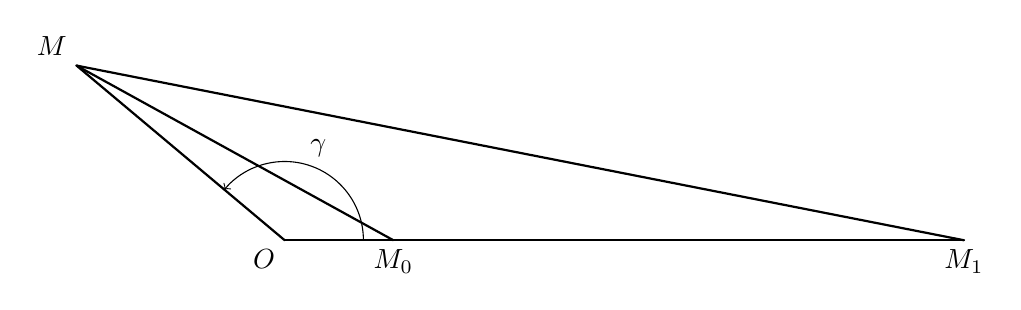
\begin{tikzpicture}[scale=1.15, line cap=round, line join=round]
\usetikzlibrary{angles,quotes}

%-----------------------
% 设定参数：保证相似的关键是 rho1 = R^2/rho0 且 |OM|=R
%-----------------------
\def\R{3.0}          % 令 OM = R
\def\rhozero{1.2}    % 令 OM0 = rho0
\pgfmathsetmacro{\rhoone}{\R*\R/\rhozero} % rho1 = R^2/rho0
\def\alpha{140}      % 令 M 在以 O 为圆心、半径 R 的某个方向上（不画圆）

%-----------------------
% 点：O, M0, M1 共线；M 满足 |OM|=R
%-----------------------
\coordinate (O)  at (0,0);
\coordinate (M0) at (\rhozero,0);
\coordinate (M1) at (\rhoone,0);
\coordinate (M)  at ({\R*cos(\alpha)},{\R*sin(\alpha)});

%-----------------------
% 画线：避免重复加粗，只画一次 OM 和 OM1(包含 OM0)
%-----------------------
\draw[thick] (O)--(M);     % 公共边 OM
\draw[thick] (O)--(M1);    % 射线 OM1（其中包含 M0）

\draw[thick] (M)--(M0);    % 小三角形第三边
\draw[thick] (M)--(M1);    % 大三角形第三边

%-----------------------
% 共用角 gamma：∠M1OM（=∠M0OM，因为 O,M0,M1 共线）
%-----------------------
\pic[draw,->,angle radius=10mm,angle eccentricity=1.25,"$\gamma$"]
  {angle = M1--O--M};

%-----------------------
% 标注点（只保留必要的）
%-----------------------
\node[below left] at (O) {$O$};
\node[above left] at (M) {$M$};
\node[below] at (M0) {$M_0$};
\node[below] at (M1) {$M_1$};

\end{tikzpicture}